\documentclass[a4paper,11pt]{article}
%\usepackage[pdftex]{graphicx}
\usepackage{amsmath}
%\usepackage[latin1]{inputenc}
%\usepackage{hyperref}
\usepackage{rotating}
\usepackage{setspace}
\usepackage{lscape}
\usepackage[round]{natbib}
\usepackage{multirow}
\usepackage{rotating}
\usepackage{vmargin}
\usepackage{epstopdf}
\usepackage{hyperref}
\usepackage{float}
\usepackage{caption}
\usepackage[tableposition=top]{caption}
%\usepackage[nolists, figuresfirst]{endfloat}
%\usepackage{sidefloat}

\setlength{\abovecaptionskip}{-8pt}

%\usepackage[usenames]{color}
%\definecolor{grey}{rgb}{0.35,0.35,0.35}
%\definecolor{webdarkblue}{rgb}{0,0,0.4}
%\definecolor{orange}{rgb}{0.7,0.2,0.05}


%\usepackage[pdfcreator={PDFLaTeX}, pdfproducer={PDFLaTeX}, pdfstartview=FitH, pdfpagemode=UseOutlines, pagebackref=false, colorlinks={true},
%citecolor={webdarkblue}, linkcolor={webdarkblue},
%urlcolor={webdarkblue}]{hyperref}



%\addtolength{\oddsidemargin}{-0.4in}
%\addtolength{\evensidemargin}{-0.4in}
%\addtolength{\textwidth}{0.8in} \addtolength{\topmargin}{-0.85in}
%\addtolength{\textheight}{1.7in}
\renewcommand{\baselinestretch}{1.2}





\setmarginsrb{2cm}{2cm}{2cm}{2cm}{0,5cm}{0,5cm}{0,3cm}{0,5cm}



% commands

\newcommand{\bi}{\begin{itemize}}
\newcommand{\ei}{\end{itemize}}
\newcommand{\be}{\begin{enumerate}}
\newcommand{\ee}{\end{enumerate}}
\newcommand{\bd}{\begin{description}}
\newcommand{\ed}{\end{description}}
\newcommand{\beqa}{\begin{eqnarray}}
\newcommand{\eeqa}{\end{eqnarray}}
\newcommand{\beq}{\begin{equation}}
\newcommand{\eeq}{\end{equation}}
\newcommand{\bs}{\bigskip}
\newcommand{\A}{$^a$}
\newcommand{\B}{$^b$}
\newcommand{\C}{$^c$}
\begin{document}



\title{\textsc{Beyond the Iceberg Hypothesis: \\Opening the Black Box of Transport Costs}} %\thanks{We are especially grateful to XXX. Part of this research was funded by the French Agence Nationale de la Recherche (ANR), under grant ANR-11-JSH1 002 01. Finally, any remaining errors are ours.}}}
%We also thank participants at the EEA 27\textsuperscript{th} Congress (Oslo), ETSG 13\textsuperscript{th} meetings (Copenhagen), INFER Workshop (Orleans), 45\textsuperscript{th} Congress of the Canadian Economic Association (Ottawa), IAW Workshop (Tubingen), and seminars at WTO, Strathclyde University, OFCE and EQUIPPE-University of Lille.
\author{Guillaume \textsc{Daudin}\thanks{%
Universit\'{e} Paris Dauphine, LEDa \& PSL, Chercheur associ\'{e} - Sciences Po (OFCE)}  \qquad J\'{e}r\^{o}me \textsc{H\'{e}ricourt} \thanks{Universit\'{e} de Lille - LEM-CNRS (UMR 9221), Universit\'{e} de Bretagne Occidentale-ICI (EA 2652) and CEPII}\qquad Lise \textsc{Patureau}\thanks{Universit\'{e} Paris Dauphine, LEDa \& PSL} }
 \maketitle

\date{July 2016}
\bigskip

\begin{abstract}
Following \cite{samuelson1954}, standard models of international trade have usually relied on modelling trade costs as an ad valorem tax equivalent. However, many common empirical facts support the existence of additive costs. This paper measures the size of additive costs in transport, using SITC 3 and 4 digit cif-fob unit values over 1974-2013 taken from US imports data. We estimate the two components of transport costs, by transport mode (air or ocean). We find that additive costs are 2.85\% of fob unit values for ocean transport costs (and ad-valorem ones 3.22\%).  These values are respectively equal to 1.9\% and 2.5\% for air transport costs. We show that taking additive costs into account improves the fit of the modelling of transport costs. The time dimension of our data allows us to characterize the evolution of transport costs. After correcting for composition effects, we obtain that all types of transport costs have been constant from 1974 to 1984 and then  decreased by 40\% over the period 1984-2013. Most of the early decline in air transport costs can be explained by the ad-valorem component. By contrast, this component nearly doubled in the 2000s. 
\end{abstract}

\thispagestyle{empty} \pagestyle{plain} \setcounter{page}{1}



{\normalsize JEL classification: F14, N70, R40\newline
Keywords: Transport costs estimates, transport costs determinants, non-linear econometrics, period 1974-2013, additive transport costs }

{\normalsize \vspace{0cm} }

{\normalsize \titlepage }

{\normalsize \newpage }

%\begin{spacing}{1.5}

\section{Introduction}


\noindent Trade costs remain central in international economic analysis. Defined as the costs associated with the exchange of goods across national borders, they are usually split into transaction costs (information costs, contract enforcement costs, costs associated with the use of different currencies...), policy costs (tariff  and non-tariff costs), time costs (time to ship goods) and transport costs \emph{per se}. Many believe that the latter have dramatically decreased with technological advance in transportation, infrastructure development and new communication technologies (see \citealp{Lafourcade_Thisse}). \citet{Glaeser04} find that, over the twentieth century, the costs of moving goods have declined by over 90\% in real terms. However, \citet{hummels2007} shows that the bulk of price declines in transportation comes from air shipping, where average cost per ton-kilometer shipped dropped by 92\% between 1955 and 2004; concerning ocean shipping, which represents the major part of world trade value, decline in trade prices are much less obvious, even if the rise in containerization lowered shipping costs from 3 to 13\%. Studies overviewed by \citet{Behar_Venables} are consistent with those results: The fall in measured transport costs has been relatively small. According to these authors, this is attributable to the growing importance of fuel costs and technical progress, which improved speed and reliability rather than decreased costs.\smallskip

Trade costs are considered as a major obstacle to international economic integration and international trade flows. According to the estimates by \citet{Jacks08}, trade cost declines explain around 55\% of the pre-World War I trade boom and 33\% of the post-World War II trade boom, while the abrupt rise in trade costs explains the inter-war trade collapse. After 1950, average trade costs fell by 16\%, notably through the reduction of policy trade costs promoted through the GATT (WTO starting in 1995) multilateral agreements. Based on panel data, \citet{novy13} thus finds  that U.S. trade costs with major trading partners declined on average by about 40 percent between 1970 and 2000. Yet, several papers (mostly based on empirical estimates of the gravity equation) have shown that trade costs (typically captured through distance) still remain a major obstacle to trade (e.g. \citealp{Head_Mayer04} and \citealp{Disdier_Head08}). \citet{anderson_wincoop_jel} estimate that average trade costs for industrialized countries put up to 170\% markups over production costs, divided into 55\% distribution costs and 74\% international costs. Within this latter dimension, 44\% are border-related trade barriers and 21\% transportation costs. \citet{Lafourcade_Thisse} also find that the share of transport costs in the consumer price of manufactured goods remains high, while \citet{Behar_Venables} obtain that the elasticity of trade with respect to freight costs is sizeable, by around -3. If much of trade-policy barriers have been removed over the second half of the 20th century, these findings suggest that the transport costs component of the overall trade costs remain large and deserve attention. This is accordingly the focus of the paper.\smallskip

Following \citet{samuelson1954}, standard models of international trade have usually relied on modelling trade costs as an \emph{ad valorem} tax equivalent (ie, as a constant percentage of the producer price per unit traded, the ``iceberg cost'' hypothesis). However, many common empirical facts support the existence of additive costs. As documented by \citet{Irrazabal_2015}, pricing structure in shipping, additive tariffs, distribution costs... often exhibit (at least partly) an additive structure. The structure (additive vs multiplicative) of transport costs is far from being anecdotal, as the literature has long pointed out its role in shaping the pattern of trade flows. The Alchian and Allen conjecture (\citealp{alchian}), which points out that the relative price of two varieties of some good will depend on the level of trade costs, does rely on the existence of additive costs: The relative demand for more expensive/higher quality product goods should increase with trade cost (``shipping the good apples out''). \citet{martin2012} gives a strong empirical support to this conjecture: Based on a very disaggregated firm-product-level database of French exporters, he finds that firms charge higher fob unit values on exports to more remote countries, whereas the iceberg hypothesis would imply the opposite. \citet{hummels_skiba} also find some strong evidence in favor of the Alchian-Allen conjecture: The elasticity of freight rates with respect to price is estimated to be well below unity, in contradiction with the iceberg assumption. Also, their estimates implied that doubling freight costs increases average fob export prices by 80-141 percent, consistent with high quality goods being sold in markets with high freight costs. \textbf{je ne sais pas quoi faire de la reference a lashkaripour. Complique d'en parler, car on ne peut pas le contredire car on n'a pas les donnees qui le permettent. Ne pas en parler? C'est un peu limite.} The existence of additive costs may also explain a large number of zeros in bilateral trade flows, and more generally, the granularity of trade flows. Relying on Spanish and US transaction-level trade data, \citet{Hornok14} find that additive trade costs of are associated with less frequent and larger shipments, i.e. more ``lumpiness'', in international trade; in other words, exporters wait to fill completely a container before sending it abroad, to decrease as much as possible the number of shipments.

%Conversely, \citet{Lashka15} finds strong empirical support for the iceberg hypothesis when considering the data at a sufficiently disaggregated level. Based on US imports data, he finds that a 10\% increase in the price of an item increases the shipping cost by 9.5\%. The additive structure of trade costs emerges only when weight is forced to be independent of price. Besides, \citet{Lashka15} supports that higher-priced, still exported to faraway markets, varieties are heavier and involve proportionally higher shipping costs, the latter increasing the relative demand for high-markup varieties. Markups would therefore be the driving force for explaining the ``shipping the good apples out'' effect in the presence of \emph{ad-valorem} trade costs.

Beyond the positive aspect of understanding trade patterns, several recent papers also point out the normative implications of additive trade costs. \citealp{sorensen2014} extends \citet{melitz}'s seminal model of international trade by including additive trade costs, in addition to the iceberg component. A key analytical result is that the welfare gain from a reduction in trade barriers is higher for a decrease in additive costs than a decrease in multiplicative costs. Calibrating on Norwegian firm-level data for 2004, \citet{Irrazabal_2015} find that an additive import tariff reduces welfare and trade by more than an identically-sized multiplicative tariff. While these results suggest that important welfare gains can be achieved by reducing additive trade costs, not much can be done in quantifying such gains though, by lack of an empirical characterization of the additive component of trade costs.\footnote{The one exception being \citet{Irrazabal_2015}, upon which we come back later.} One objective of the paper is to palliate this gap. \bigskip


Our paper contributes to the literature by providing results on the size of transport costs over time, explicitly distinguishing between multiplicative and additive parts. More precisely, we provide estimates of the relative importance of additive and multiplicative transport costs over several decades. To do so, we update the detailed US customs, sector-level data from the US Imports of Merchandise used by \citet{hummels2007}, to cover the period from 1974 to 2013. Closely related to this paper is the work by \citet{Irrazabal_2015}, which develop a structural framework for inferring additive trade costs from firm-level trade data. Based on Norwegian firm-level data, their results suggest that additive costs are on average 30-45\% relative to the median consumer price, and that they are strongly correlated with standard proxies for trade costs (like e. g., distance). However, while our data requires that we only consider transportation costs, our approach departs from theirs in several key aspects.

First, our theoretically agnostic approach provides a fairly simple framework for assessing \emph{both} multiplicative and additive parts of transportation costs, which may prove to represent a non-negligible advantage for calibrating related models. We thus obtain that the mean values over 1974-2012 of iceberg costs are equal to 2.5\% in air and 3.2\% in ocean shipping, whereas the additive component amounts to 1.9\% and 2.85\% of the fob price in air and ocean shipping respectively. To our best knowledge, our paper is the first to provide such an extensive quantitative assessment of the magnitude of both multiplicative and additive costs in total transport costs. Second, we provide, through standard measures of ``goodness-of-fit'', an empirical assessment of what standard international trade models lose by skipping additive transport costs. Quantitatively, the omission of the additive term leads to overestimate the iceberg component by roughly a factor 2. On average over the whole period, biased estimate for iceberg is 5\% for Air and 6\% for Vessel, while unbiased estimate is respectively 2.5\% and 3.2\%. Third, the time dimension of our data allows us to characterize the evolution of transport costs, by transport mode (air or vessel) and for each specific (multiplicative and additive) cost over a forty years time span. After excluding the composition effects, we obtain that transport costs \textit{per se} have roughly decreased by 40\% over the period 1974-2012. Decomposing by transport mode and by type of transport costs allows to go deeper into this picture. First, as in \cite{hummels2007}, we find that the transport costs decrease is more pronounced in air than in ocean shipping, starting in 1984. However, while ocean shipping costs display a regular decreasing pattern until 2012, air transport costs rather get stabilized over 2005-2012. Second, while both the additive and multiplicative components of ocean transport costs have roughly decreased by 40\% over the period, air transport costs exhibit more contrasted trends. If the reduction of air shipping costs can most be attributed to the decrease in its multiplicative component over 1974-2005, the opposite scheme prevails afterwards, the reduction in per-unit air transport costs being compensated by an increase in the ad-valorem component. \smallskip


Section \ref{sec:data_method} explains the data sources and the empirical methodology retained in the paper. Sections \ref{sec:results_decomposition} and \ref{sec:results_trends} report our results. In Section \ref{sec:results_decomposition}, we characterize the role of the additive component of transport costs. After reporting the mean values over the period (by transport mode), we show the improved performance in including additive trade costs in the measure of transport costs. This being established, Section \ref{sec:results_trends} characterizes the trends in each component of transport costs (by transport mode) over the period 1974-2012. Section \ref{sec:conclu} concludes.



\section{Data Sources and Empirical Methodology \label{sec:data_method}}

\subsection{A measure of Transportation Costs}

As in \cite{hummels2007} (among others), our measure of transportation costs consists in exploiting the difference between commodity-level export and import prices.
We first use values, quantities and freight costs to recover free-on-board (FOB) and cost-insurance-fret (CIF) prices, by goods, country of origin and transportation mode. More precisely, the (unit) FOB price is computed as the total customs value divided by the shipping weight; in other words, it is the price for the good net of transportation costs. The CIF price is then computed as the sum of the customs value and freight charges, once again divided by the shipping weight. Our dependant variable is finally computed as the ratio of the CIF price divided by the FOB price. Strictly higher than 1, the variable provides therefore with a measure of transport costs as a proportion of the good's price, an \emph{ad valorem} equivalent.

The database we use to construct our measure of transport comes from US annual Imports of Merchandise provided by the Census bureau\footnote{More information available at: \url{http://www.census.gov/foreign-trade/reference/products/catalog/fl_imp.txt}}, spanning from 1974 to 2013. Using this dataset has (at least) three main advantages. First, this dataset has been used by \cite{hummels2007}, which enables us to compare our results to his findings. However, we complement Hummels' (2007) findings as we extend the time coverage to 2013 (while \cite{hummels2007} stops in 2004). As we show in Section \ref{sec:results_trends}, extending the time period over he recent years delivers interesting insights regarding the trends in air shipping costs. Second, and importantly, this dataset delivers a strong statistical reliability arising from a single, trustworthy customs origin. Based on customs declarations, this dataset inventories all imports (both values and quantities) by origin to the United states at the HS 10-digit highly disaggregated level, with a concordance code to the SITC 5-digit coding system. In addition, the database reports information regarding freight expenditures and transportation mode (Ocean Vessel and Air). The first will be crucial to compute transport costs (see below), the second will allow us enlightening substantial differences in the dynamics of transport costs across transportation mode. Third, using this dataset allows us to have the import price of the good (CIF price), next to the export price (FOB price). This is highly valuable, as we can estimate both the \textit{levels} of the iceberg trade costs and of the additive trade costs. This differentiates us from \citet{Irrazabal_2015}, which can only estimate the ratio of additive costs as a share of the total consumer price (the only price they can encover).

It is also true that using this dataset has drawbacks. First, our measure of the cif-fob price gap only covers transportation costs by nature, thereby being mute about the others dimensions of international trade costs, unlike \citet{Irrazabal_2015}.  Further, in terms of transport costs \textit{per se}, this measure being based on freight costs, omits the other dimension of transport costs related to the time value of goods in transit. According to \citet{anderson_wincoop_jel}), the 21\% markup over production costs coming from transport costs includes both directly measured freight costs and 9\% tax equivalent of the time value of goods in transit. \textbf{en faire un contre-argument positif}

Even if the data of transportation costs is available at a more disaggregated level, we use sectorial price data at the 3-digit level, primarily for technical reasons. As detailed below, the use of a nonlinear estimator triggers computational limitations that do not make them a likely option, especially when covering a long period of time. Yet, we ensure the robustness of these results by conducting the estimations at the 4-digit level (for some selected years). Comparing different levels of aggregation is useful to check differences and the presence of biases precisely due to aggregation. Depending on the considered year, this leaves us with around 200 (3-digits) and 600-700 (4-digits) products, from approximately 200 countries of origin.


\subsection{Empirical specification}

\paragraph{The estimated equation} Our purpose is to provide estimates over time of the sizes of multiplicative and additive costs among total transport costs. To do so, we start from a very simple equation (similar to \cite{Irrazabal_2015} or \cite{martin2012}, among others):

\begin{equation}
p = \tau \widetilde{p} + t \label{eq:base}
\end{equation}

\noindent This equation expressed the consumer (import, or cif) price $p$ as a function of the producer (export, or fob) price $\widetilde{p}$ given both per-unit ($t$) and ad-valorem ($\tau$) transport costs. As usual in the literature, the so-called ``iceberg'' trade costs are denoted $\tau$ (with $\tau=1$ meaning no iceberg trade costs), while additive trade costs are labeled $t$ (with $t=0$ implying no additive trade costs). We estimate this equation for each year over the period 1974-2013, and for each of the two transportation modes reported (air or vessel), on a sectoral-origin country basis. Let us denote $i$ the origin country, and $k$, the sector (or product). Transforming the above equation (\ref{eq:base}) as ratio, we thus get the equation to be estimated as given by:\footnote{Also keeping in mind that the estimated equation is transport-mode and year specific (air or ocean shipping). We skip the year and transport-mode dimensions here to alleviate notations.}

\begin{equation}
\frac{p_{ik}}{\widetilde{p}_{ik}} -1 = \tau_{ik} -1 +\frac{t_{ik}}{ \widetilde{p}_{ik}} \label{eq:base_estimee}
\end{equation}


\paragraph{Estimation Strategy} We follow \citet{Irrazabal_2015} by considering that \textit{1°)} both multiplicative and additive costs are separable between the origin country ($i$) and the product ($k$) dimensions, and \textit{2))} in a multiplicative way for the former and an additive way for the latter. In other words, $\tau_{ik}$ and $t_{ik}$ from Equation (\ref{eq:base_estimee}) become:

\begin{eqnarray}
\tau_{ik} &=& \tau_{i} \times \tau_{k} \label{eq:iceberg}\\
t_{ik} &=& t_{i} + t_{k} \label{eq:add}
\end{eqnarray}


As a result, our underlying theoretical equation is specified as:

\begin{equation}
\frac{p_{ik}}{\widetilde{p}_{ik}}-1 =\tau_{i} \times \tau_{k} -1 +\frac{t_{i} + t_{k}}{ \widetilde{p}_{ik}} \label{eq:theory_equation}
\end{equation}

The ratio $\frac{p_{ik}}{\widetilde{p}_{ik}}$ has a ``one-lower bond'', since by construction, the \emph{cif} price $p$ cannot be lower than the \emph{fob} price: $p>\widetilde{p}_{ik}$. Taking into account this constraint in the estimation requires to impose a multiplicative structure for the error term, according to:

\begin{equation*}
\frac{p_{ik}}{\widetilde{p}_{ik}}-1 =\left(\tau_{i} \times \tau_{k} -1+\frac{t_{i} + t_{k}}{\widetilde{p}_{ik}} \right)\times \varepsilon_{ik}
\end{equation*}

Taking in log, this finally drives us to estimate the following equation:

\begin{equation}
\ln\left(\frac{p_{ik}}{\widetilde{p}_{ik}}-1 \right)= \ln \left(\tau_{i} \times \tau_{k}+\frac{t_{i} + t_{k}}{\widetilde{p}_{ik}}-1 \right) + \epsilon_{ik} \label{eq:estimatedequation}
\end{equation}
where $\tau_{i}$, $\tau_{k}$, $t_{i}$ and $t_{k}$ are the parameters to be estimated, i.e., fixed effects specific to each origin country $i$ and sector $k$, and $\epsilon_{ik}= \ln(\varepsilon_{ik})$.


The shape of our main equation \ref{eq:estimatedequation} is such that estimations cannot be performed using standard linear estimators. Therefore, all estimates are performed using non linear least squares. The basis of the method is to approximate the model by a linear one and to refine the parameters by successive iterations. The intuitive criterion for convergence is that the sum of squares does not decrease from one iteration to the next. In our case, due to computational limitations implied by the size of our dataset, we implement 100 iterations and set the convergence criterion for successive parameter estimates and for the residual sum of squares at 0.01. Finally, to eliminate the potential influence of outliers, we excluded observations in the 5 percent from the upper and lower tails of the distribution in the regression variables, and all our three measures of trade costs are bounded by 0 as minimal value. These cut-offs are aimed at eliminating reporting or coding errors.\medskip


Further, one key objective of the paper is to characterize the importance of additive costs relatively to iceberg costs. Put differently, what traditional models of international trade lose by ignoring additive costs? A natural way to answer this question is to perform estimations of equation (\ref{eq:estimatedequation}) constraining $t$ to be equal to zero, and compare the fitting properties and the explanatory power of the restricted and complete models. This is done by computing several standard diagnostic statistics (R$^{2}$ and statistics based on the likelihood function). Accordingly, for each year and transport mode, we estimate two equations, depending on additive transport costs being included (Equation (\ref{eq:model_with_add}) or not (Equation (\ref{eq:model_nlI})):

\begin{eqnarray}
\ln\left(\frac{p_{ik}}{\widetilde{p}_{ik}}-1 \right)&=& \ln \left(\underbrace{\tau_{i} \times \tau_{k}}_{\tau^{ice}_{ik}}-1 +\underbrace{\frac{t_{i} + t_{k}}{\widetilde{p}_{ik}}}_{t^{add}_{ik}} \right) + \epsilon_{ik} \label{eq:model_with_add} \\
\ln\left(\frac{p_{ik}}{\widetilde{p}_{ik}}-1 \right)&=& \ln \left(\underbrace{\tau_{i} \times \tau_{k}}_{\tau^{nlI}_{ik}}-1 \right) + \epsilon^{nlI}_{ik} \label{eq:model_nlI}
\end{eqnarray}

After estimating Equation (\ref{eq:model_nlI}), we can re-built a measure of each component $\widehat{\tau}^{ice}_{ik} = \widehat{\tau_{i}} \times \widehat{\tau_{k}}$ and $\widehat{t}^{add}_{ik} = \widehat{t}_{i} + \widehat{t}_{k}$, that is country-product specific, by year and transport mode. When assuming iceberg costs only (Equation (\ref{eq:model_nlI}), we proceed similarly to get $\widehat{\tau}^{nlI}_{ik} = \widehat{\tau_{i}} \times \widehat{\tau_{k}}$.\footnote{In this case, notice that the equation could be estimated relying on a non-linear form. To preserve comparability of the results, we keep the same non-linear estimation method in both cases though.} Still following \citet{Irrazabal_2015}, we take the average over the product-country dimension, using the values of each trade flow ($ik$-specific) over total yearly trade as a weighting scheme. We thus recover a ``synthetic estimate'' of each type of transport cost $\widehat{\tau}$ and $\widehat{t}$, for each year and transportation mode. These results are reported in Section \ref{sec:results_decomposition}.


\section{Decomposing Transport Costs: The importance of the additive component \label{sec:results_decomposition}}

The objective of this section is twofold. First, we characterize the magnitudes of transport costs over time (by transport mode), distinguishing whether the additive component $t_ik$ is included or not in the estimated equation (\ref{eq:estimatedequation}). Second, we quantitatively assess the importance of the per-unit component of in overall transport costs through the means of goodness-of-fit measures.


\subsection{Decomposing transport costs over 1974-2013}

Our first contribution to the literature is to provide estimates for the size of both the multiplicative and the additive components of transport costs. Tables \ref{tab:result_air} and \ref{tab:result_ves} report a summary of our results. Precisely, they display the mean and median values of each type of trade costs (multiplicative estimated alone, estimated along with additive costs and the additive component), expressed in percentage of the fob price, as well as the associated standard deviation, averaged over the period 1974-2013 and for selected years.

\begin{table}[htbp]
  \centering
  \caption{Air (3 digits): Mean values over the period and selected years}
\begin{center}
    \begin{tabular}{lccccccc}

  %  \toprule
   \hline\hline
          & \multicolumn{6}{c}{Year}                      &  \\

          & 1974  & 1980  & 1990  & 2000  & 2010  & 2013  & \multicolumn{1}{c}{\textbf{Mean stat}} \\
 \hline
\multicolumn{1}{l}{\textbf{With only Iceberg Trade Costs}} &       &       &       &       &       &       & \multicolumn{1}{c}{\textbf{}} \\
Mean  & 6.9 & 5.4 & 5.0 & 3.6 & 4.2 & 3.4 & \multicolumn{1}{c}{\textbf{5.1}} \\
Median & 5.4 & 3.8 & 4.4 & 2.5 & 3.4 & 2.9 & \multicolumn{1}{c}{\textbf{4.2}} \\
Standard Error & 0.052 & 0.049 & 0.039 & 0.033 & 0.037 & 0.024 & \multicolumn{1}{c}{\textbf{0.042}}\\
\hline
\multicolumn{1}{l}{\textbf{With Additive \& Iceberg Trade Costs }} &       &       &       &       &       &       & \multicolumn{1}{c}{\textbf{}}\\
\multicolumn{1}{l}{\textit{Additive term }} &       &       &       &       &       &       & \multicolumn{1}{c}{\textbf{}} \\
\multicolumn{1}{l}{Mean } & 2.6 & 2.0 & 1.8 & 1.3 & 1.1 & 1.0 & \multicolumn{1}{c}{\textbf{1.9}} \\
\multicolumn{1}{l}{Median} & 1.1 & 0.5 & 0.8 & 0.5 & 0.4 & 0.5 & \multicolumn{1}{c}{\textbf{0.7}} \\
\multicolumn{1}{l}{Standard Error} & 0.040 & 0.041 & 0.033 & 0.028 & 0.024 & 0.020 & \multicolumn{1}{c}{\textbf{0.076}} \\
\multicolumn{1}{l}{\textit{Iceberg term}} &       &       &       &       &       &       & \multicolumn{1}{c}{\textbf{}} \\
\multicolumn{1}{l}{Mean } & 3.6 & 2.3 & 2.4 & 1.7 & 2.6 & 1.7 & \multicolumn{1}{c}{\textbf{2.5}} \\
\multicolumn{1}{l}{Median} & 2.7 & 1.6 & 1.6 & 1.2 & 2.2 & 1.7 & \multicolumn{1}{c}{\textbf{1.8}} \\
Standard Error & 0.032 & 0.025 & 0.021 & 0.016 & 0.023 & 0.012 & \multicolumn{1}{c}{\textbf{0.023}} \\
\hline
\# observations & 14955 & 16118 & 24958 & 35027 & 40279 & 39351 & \textbf{} \\
\hline\hline
    \end{tabular}%
  \end{center}
  \label{tab:result_air}%
\tiny{Statistics are obtained weighting each observation by its value in transport (mode-dependent). Mean and median values of all type of transport costs are expressed in percentage of the fob price. }
\end{table}%


\begin{table}[htbp]
  \centering
  \caption{Vessel (3 digits): Mean values over the period and selected years}
\begin{center}
    \begin{tabular}{lccccccc}

  %  \toprule
   \hline\hline
          & \multicolumn{6}{c}{Year}                      &  \\

          & 1974  & 1980  & 1990  & 2000  & 2010  & 2013  & \multicolumn{1}{c}{\textbf{Mean stat}} \\
 \hline
   \textbf{With only Iceberg Trade Costs} &       &       &       &       &       &       & \textbf{} \\
Mean  & 9.8 & 6.5 & 5.7 &5.1 & 4.0 & 3.6 & \textbf{5.8} \\
Median & 9.6 & 5.5 & 4.6 & 4.9 & 3.6 & 3.3 & \textbf{5.1} \\
Standard Error & 0.053 & 0.040 & 0.032 & 0.028 & 0.020 & 0.018 & \textbf{0.032} \\
\textbf{With Additive \& Iceberg Trade Costs} &       &       &       &       &       &       & \textbf{} \\
\hline
\textit{Additive term } &       &       &       &       &       &       & \textbf{} \\
Mean  & 5.1 & 3.4 & 2.7 & 2.8 & 2.5 & 1.5 & \textbf{2.9} \\
Median & 2.9 & 2.3 & 1.7 & 2.2 & 1.9 & 0.8 & \textbf{1.9} \\
Standard Error & 0.085 & 0.046 & 0.040 & 0.043 & 0.025 & 0.020 & \textbf{0.041} \\
\textit{Iceberg term} &       &       &       &       &       &       & \textbf{} \\
Mean  & 5.4 & 3.1 & 3.3 & 2.5 & 1.9 & 2.2 & \textbf{3.2} \\
Median & 4.9 & 2.4 & 2.8 & 2.1 & 1.8 & 1.8 & \textbf{2.8} \\
Standard Error & 0.041 & 0.023 & 0.022 & 0.021 & 0.018 & 0.018 & \textbf{0.028} \\
\hline
\# obs & 19007 & 17356 & 28383 & 36090 & 37748 & 38473 & \textbf{} \\
\hline\hline
    \end{tabular}%
  \end{center}
  \label{tab:result_ves}%
\tiny{Statistics are obtained weighting each observation by its value in transport (mode-dependent). Mean and median values of all type of transport costs are expressed in percentage of the fob price.}
\end{table}%

Tables \ref{tab:result_air} and \ref{tab:result_ves} yield the following results. First, the magnitude of overall transport costs is sizeable, either considering the average value over the period or even in the most recent years. Over 1974-2013, they correspond to a mean increase of the export price by 5.8\% for ocean shipping, and by 5?1\% for air shipping. \textbf{comparer avec la litterature?}

\subsection{Asessing the importance of per-unit trade costs}
In this section, we investigate the properties of our two models (with and without an additive term), to assess what loss of explanatory power is implied by the omission of the additive term. We start with a simple visual inspection of Figure \ref{fig:good_fit}, where are reported the yearly median \emph{ad valorem} estimates of the iceberg costs ($\widehat{\tau}_{i}$) estimated in equation \ref{eq:estimatedequation}\footnote{Qualitatively similar results are obtained when the mean values are reported instead. More details of those results available upon request to the authors.}. The dotted line plots the estimated iceberg cost ($\widehat{\tau}^{nlI}$) when the additive term $t$ is restricted to 0 (Equation (\ref{eq:model_nlI}) being estimated), and the plain dark line represents the iceberg cost in the model including a non-null additive term (Equation (\ref{eq:model_with_add}) being estimated). In both cases, multiplicative costs are reported minus one, for a better reading comfort and comparability with Figure \ref{fig:mult_vs_add}.


\begin{figure}[htbp]
\caption{Multiplicative Costs (-1), Median Value 3 digits}\label{fig:good_fit}
\begin{center}
\begin{tabular}{cc}
{\small (a) Air } & {\small (b) Vessel}\\
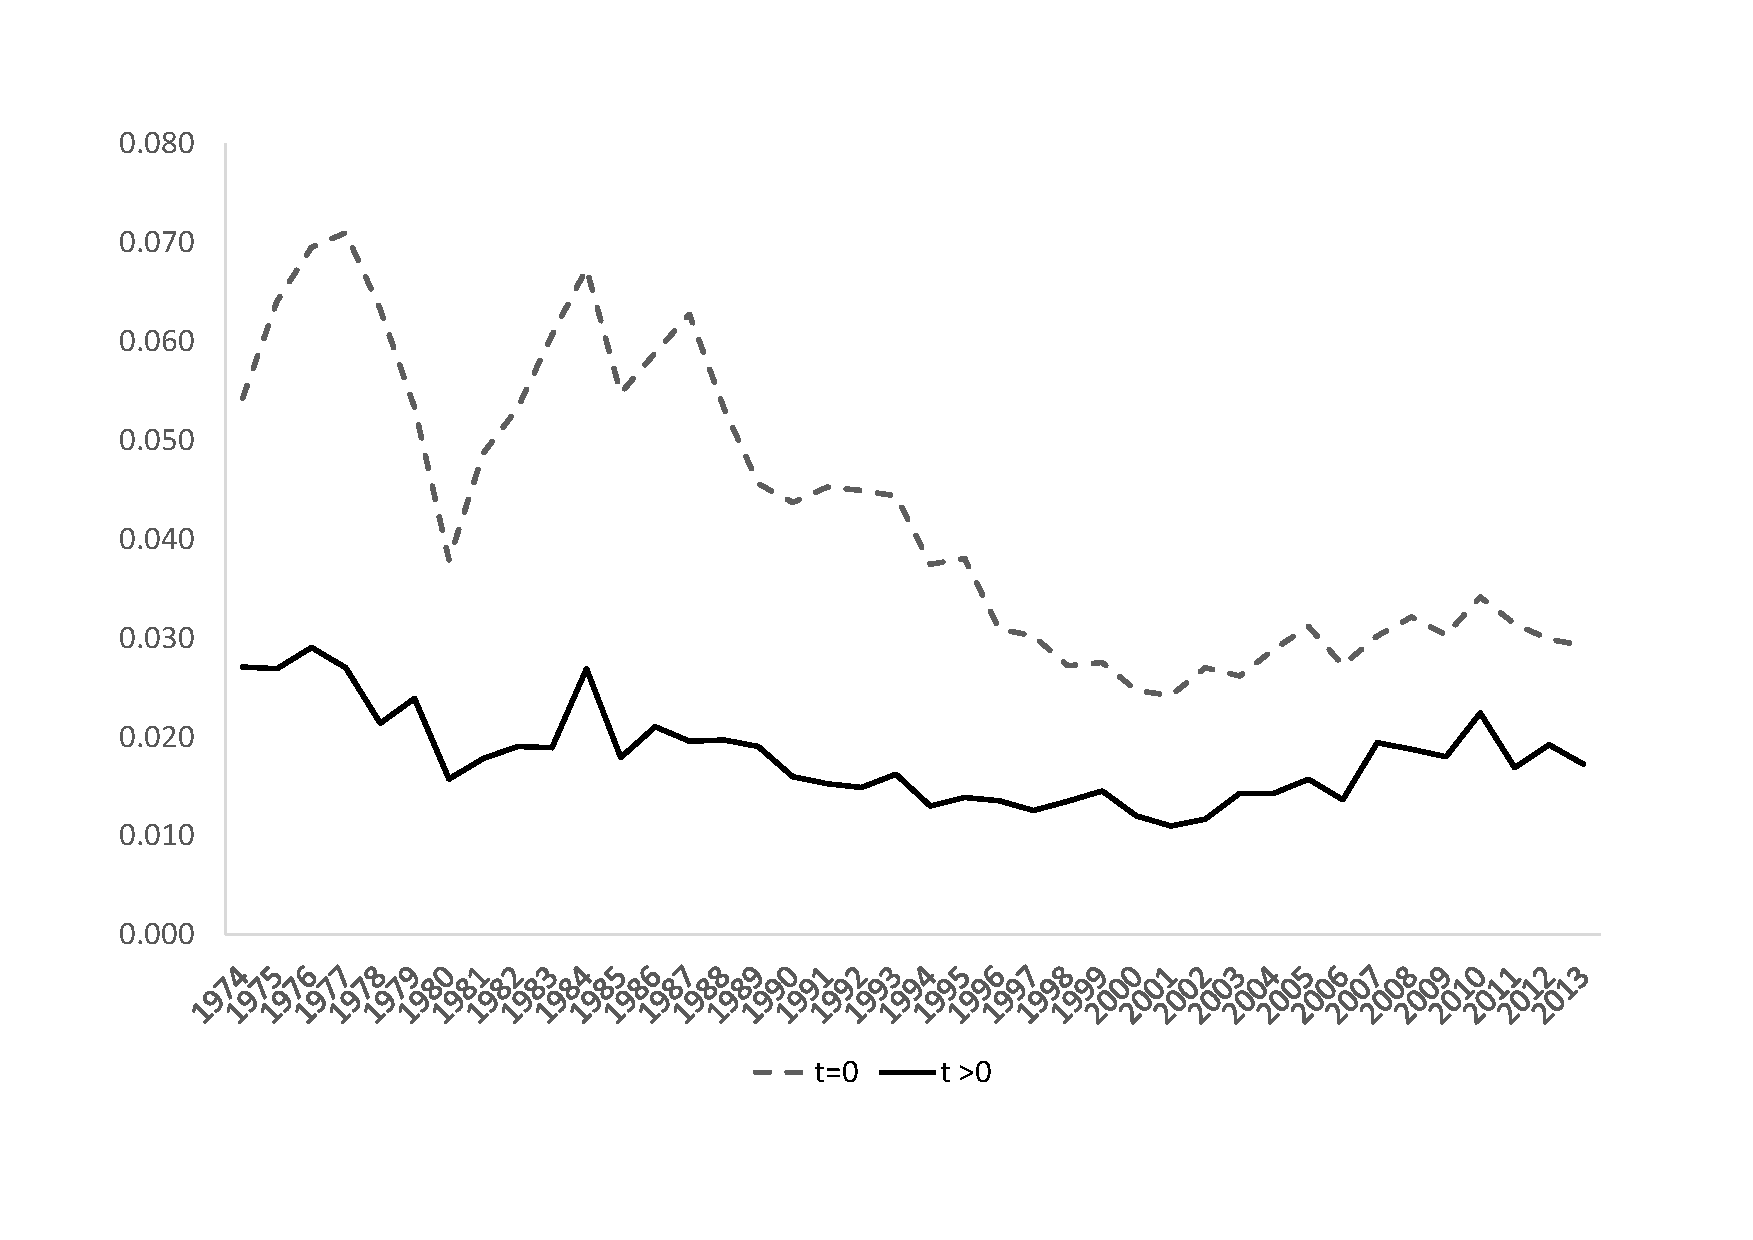
\includegraphics[width=3.5in, height=3in]{graph1a.pdf}
& 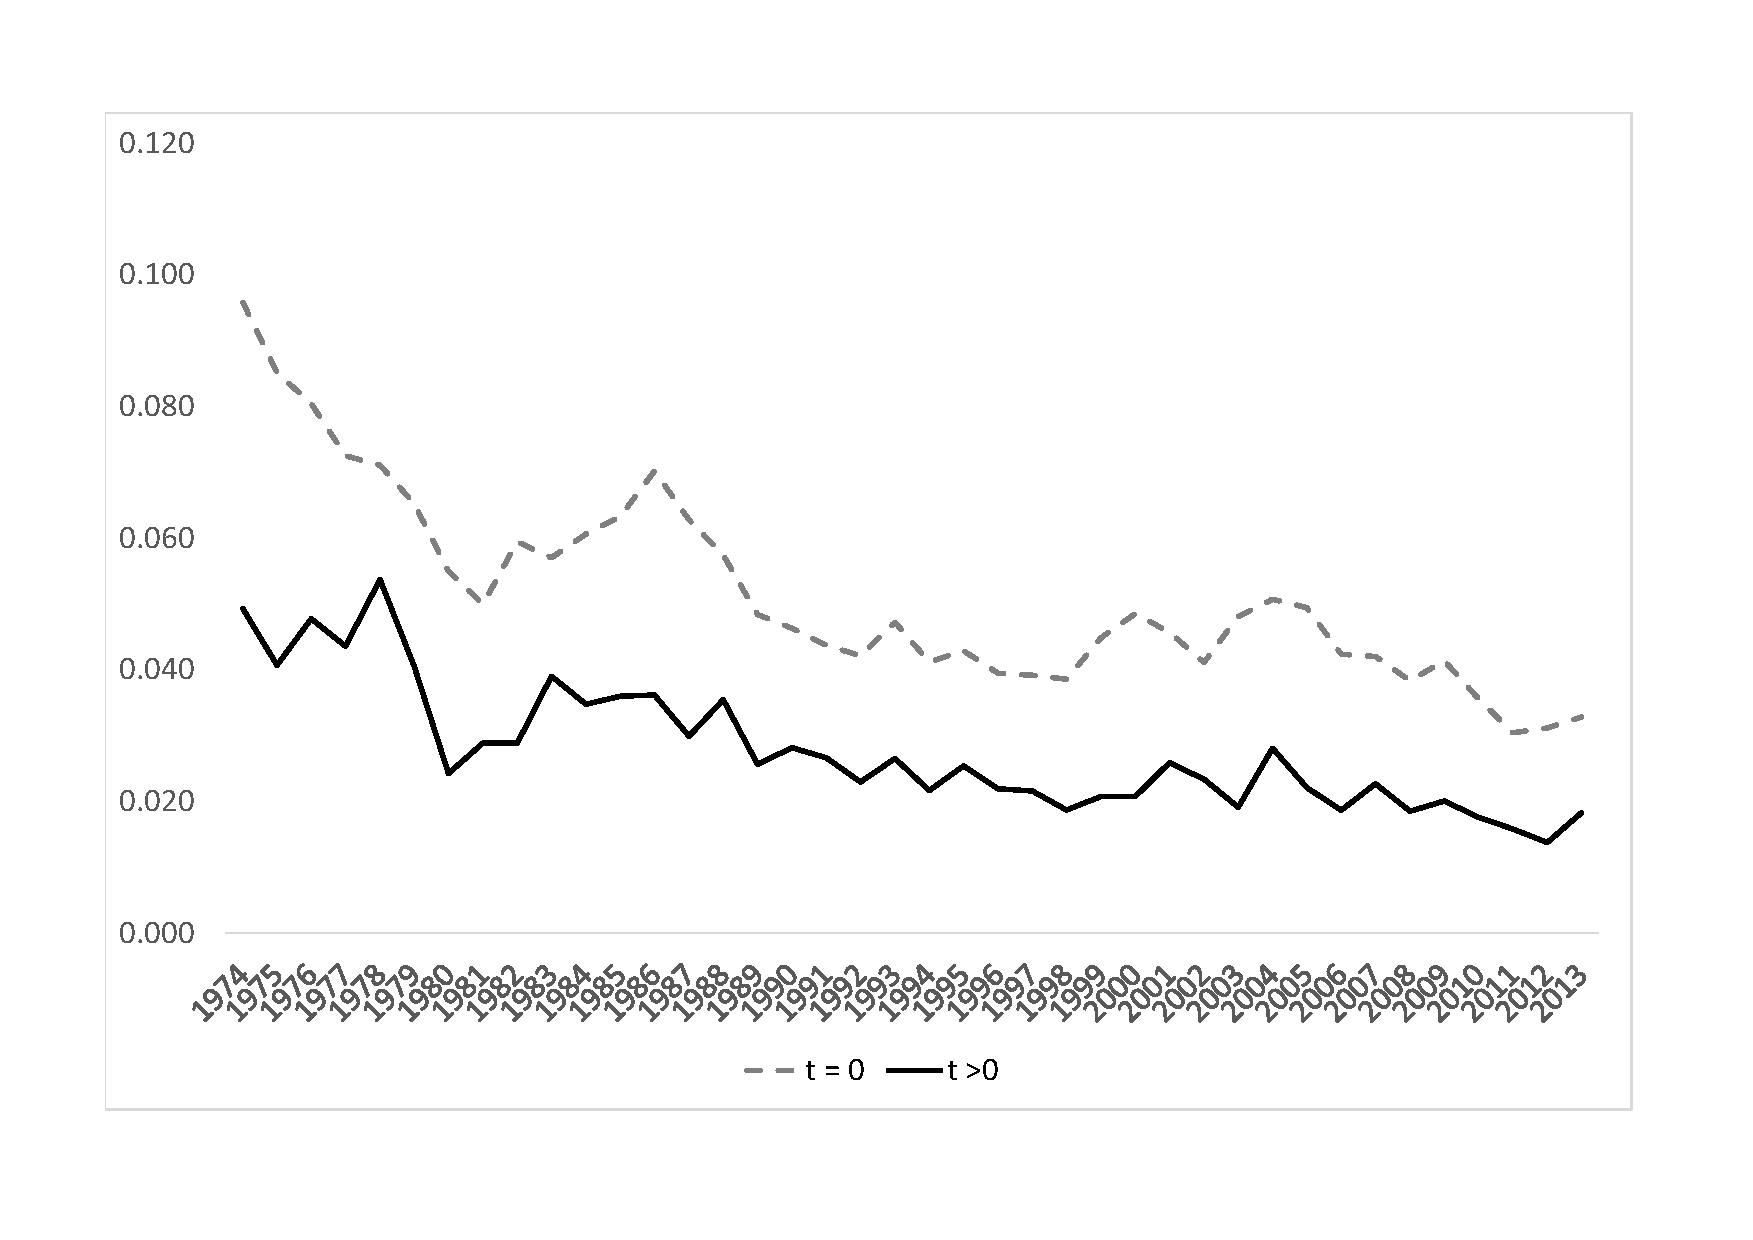
\includegraphics[width=3.5in,height=3in]{graph1b.pdf} \\
\end{tabular}
\end{center}
\end{figure}

In Figure \ref{fig:mult_vs_add}, we report the yearly median value for each component of transport cost (expressed in terms of the fob price, by transport mode) ) after running estimation of Equation (\ref{eq:model_with_add}). 

%Economic interpretation
%usepackage{float} + H is great to keep images on the right page
\begin{figure}[H]
\caption{Multiplicative vs. Additive Trade Costs, Median Value 3 digits}\label{fig:mult_vs_add}
\begin{center}
\begin{tabular}{cc}
{\small (a) Air } & {\small (b) Vessel}\\
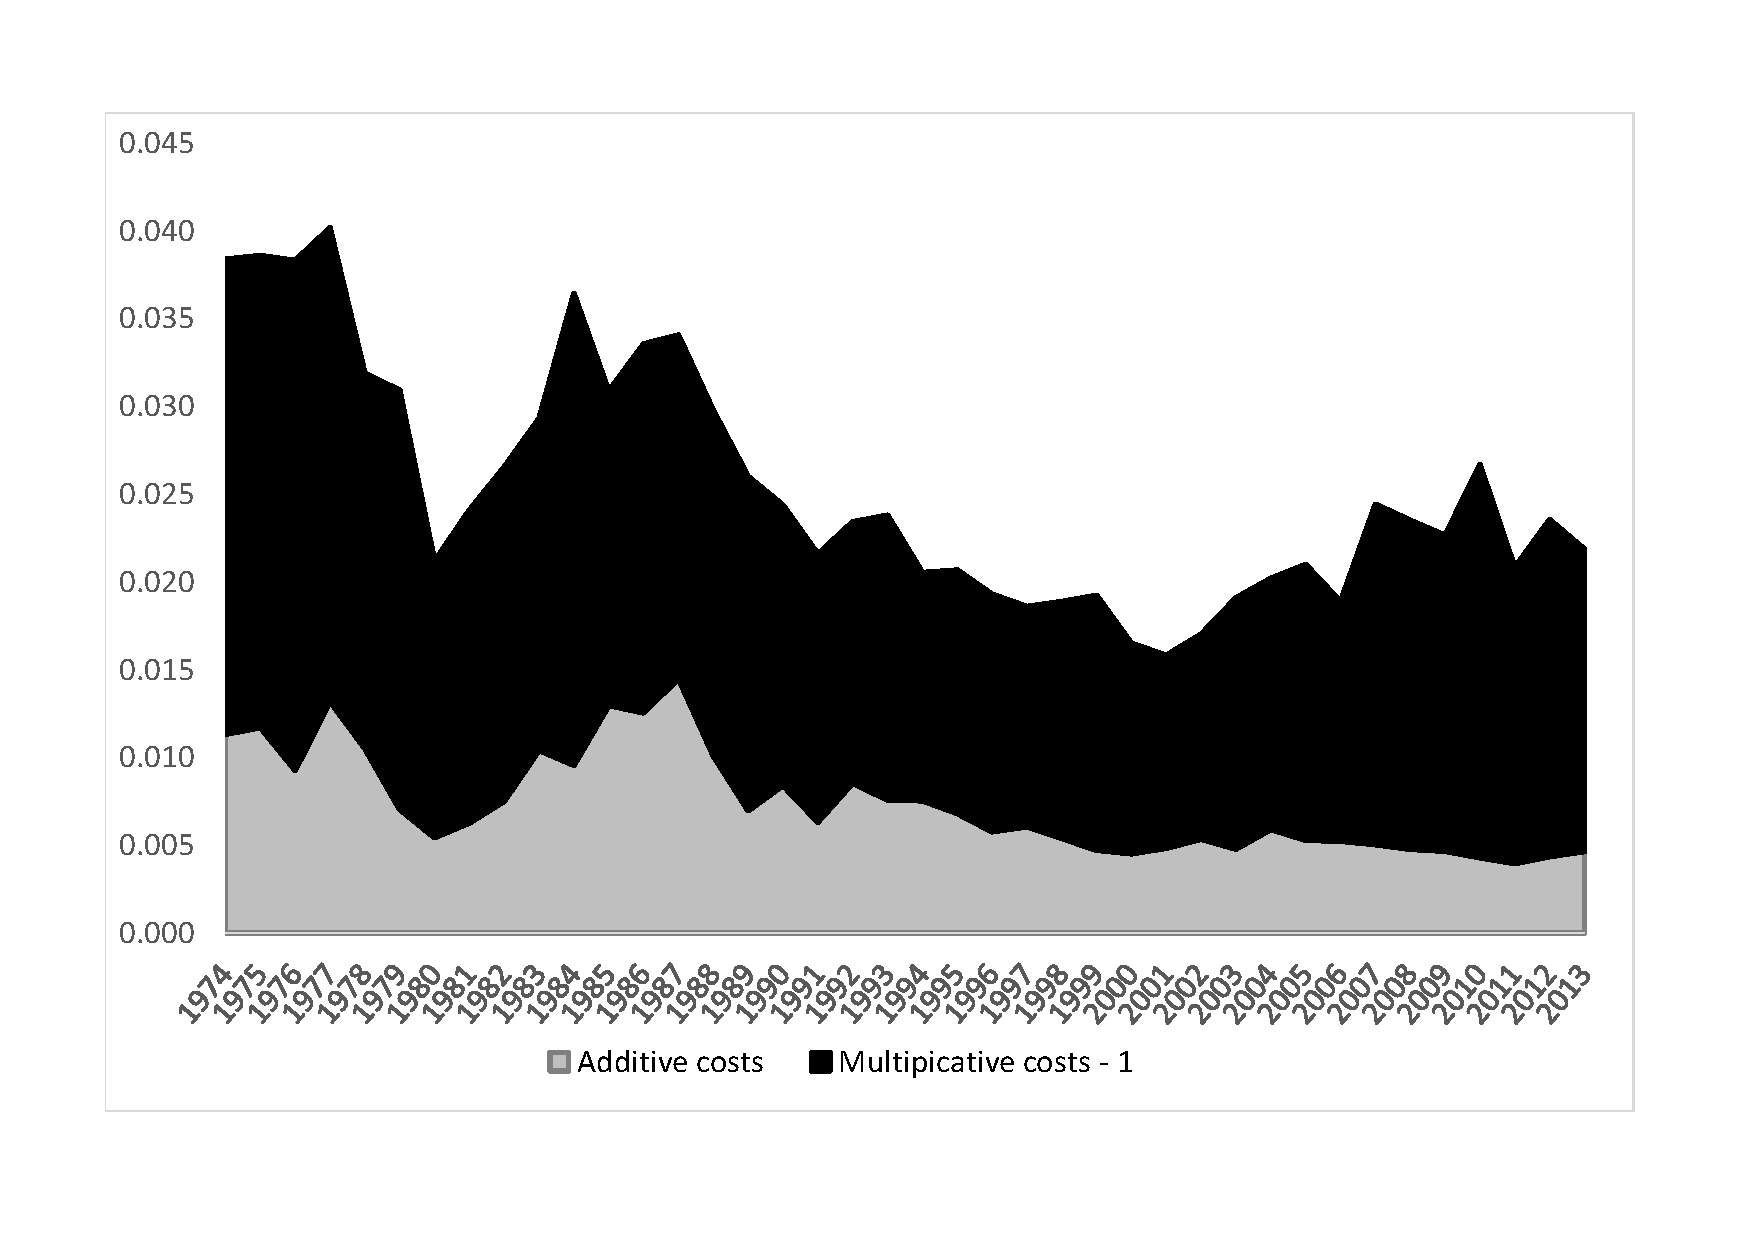
\includegraphics[width=3.5in, height=3in]{graph2a.pdf}
& 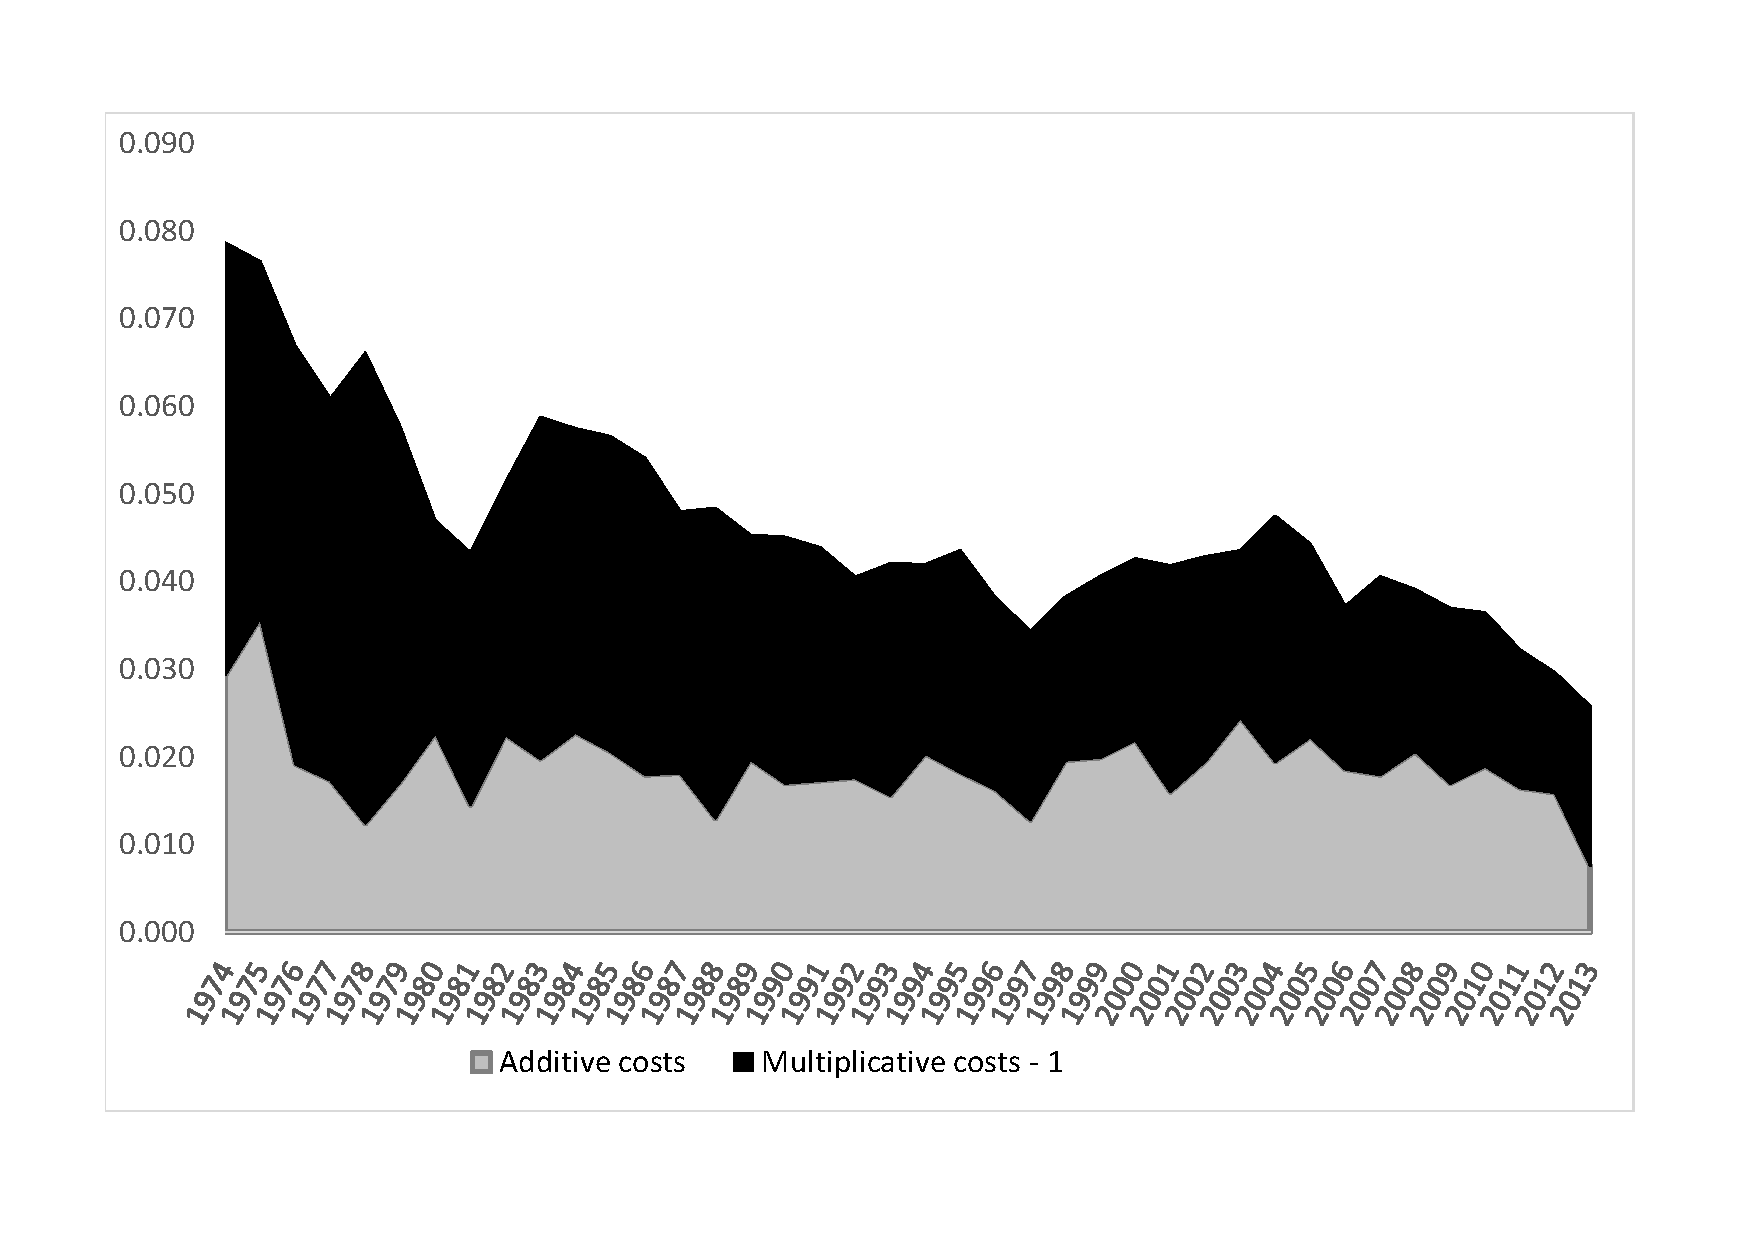
\includegraphics[width=3.5in,height=3in]{graph2b.pdf} \\
\end{tabular}
\end{center}
\end{figure}



For both transport modes, we can infer from Figure \ref{fig:good_fit} that the omission of the additive term seriously biases the multiplicative term upward. For Air, the size of the bias seems to decrease over time, while it seems pretty stationary for Vessel. In any case, the omission of the additive term leads to overestimate the iceberg component by roughly a factor 2. 

In order to deliver a more systematic diagnosis, we use several standard measures of fit. Of course R$^{2}$ comes naturally to mind, but its use is far from being straightforward when evaluating non-linear estimates.\footnote{R-squared is based on the underlying assumption that the adjusted model is a linear one. In a non-linear context, R-squared is therefore inappropriate, strictly speaking. However, if the error distribution is approximately normal, a standard metric like R-squared remains informative on the quality of adjustment.)}. Therefore, we provide as a complement the Standard Error of Regression (SER) which represents the average distance that the observed values fall from the regression line. Smaller values are better because it indicates that the observations are closer to the fitted line. We also report the log-likelihood function, and two measures derived, the Akaike Information Criterion (AIC) and the log-likelihood (LL) ratio test. A decrease in the log-likelihood function points to a better quality-of-fit. However, the likelihood function systematically decreases with the number of parameters included; the AIC criterion allows for correcting this overfitting by including a penalty in the computation of the statistic, so that AIC stat $= 2 \times \textrm{number of parameters} - 2 \times \textrm{Likelihood} $. Once again, the preferred model is the one with the minimum AIC value. Finally, the log-likelihood ratio test statistic compares systematically the likelihood of the Unrestricted model (\emph{UR}, including an additive term, see equation~\ref{eq:estimatedequation}) and the Restricted one (\emph{R}, i.e. equation~\ref{eq:estimatedequation} with $t=0$). The null tested is that the two models are statistically equivalent. Results are reported in Tables~\ref{tab:good_fit_air} and \ref{tab:good_fit_ves}.



%If we keep the R² as a measure of GoF, we will have to provide some evidence of normality for residuals. In addition, a plot of observations and the adjustment curve might be useful.
Unsurprisingly, it appears that the inclusion of the additive term leads to an improvement of the quality of fit, whatever the considered criterion or transport mode. On average over the whole period, $R^{2}$ doubles when restricting to Air Transport, and increases by 50\% for Vessel. Similar qualitative conclusions arise from the comparisons of SERs, but may be more reliable on the quantitative side, since the use of R-squared on non-linear estimates may be qualified. Regarding the other criteria, improvements allowed by the inclusion of the additive term are roughly of the same extent across transport modes. Both AIC and Log-Likelihood statistics decrease with the inclusion of the additive term, and the LL test unambiguously reject the null of statistical equivalence of the two models. This is true whatever the considered year.

However, going into the examination of the levels of these goodness-of-fit statistics reveals intriguing differences. Multiplicative costs appear more important for the Vessel sector, where they account for 39\% of the variance of the CIF/FOB ratio, versus 31\% for the Air sector; the standard error of the regression based only on the iceberg term is consistently lower for Vessel than for Air. Besides, the dynamics over time also reveals intriguing differences. Quality of fit decreases strongly after 2000, for both transport modes. For Air, it seems that the additive term explains less and less variance over time: in 2000, the inclusion of the additive term allows adding more than 30\% of explanatory power, and decreases the SER by 14 percentage points ;  in 2010 and 2013, it is hardly more than 10\% for the $R^{2}$, and 7 percentage points for the SER. The picture is quite different for Vessel. For that transport mode, the inclusion of the additive term increases the R$^{2}$ by a percentage very similar whatever the considered year (between 12 and 18\%); a similar conclusion can be drawn for the SER, which decreases by 8-11 percentage points across the years. It appears that the deteriorating performance of the model in terms of goodness-of-fit from 2000 comes mainly from the decreasing performance of the iceberg term. In order to enlighten the roots of these differences, the following section elaborates further on the quantitative dynamics of each type of cost.

For comparison purposes, we provide in the appendix similar results for some years based on a more disaggregated dataset at the product level (4-digits).\footnote{Since we use a non-linear estimator, estimations are highly computer-intensive. This explains why we decided to focus on the 3-digit product classification, which requires less time-consuming calculations.}. If anything the quality of fitting appears slightly higher when estimations are based on the 4-digits classification. This is especially true for the model restricting trade cost to their iceberg dimension, whatever the transport mode considered. When the additive part is taken into account however, the difference becomes very small, whatever the considered criterion.

Using a more disaggregated classification unsurprisingly adds some statistical precision, but not to an extent which disqualifies the use of slightly more aggregated data.
% need for SER on all years to be complete.


\subsubsection{Interpretation}

We now more specifically investigate the long-run behavior of the estimated iceberg and additive parameters. Tables \ref{tab:result_air} and \ref{tab:result_ves} report, respectively for the Air and Vessel sector, our estimates for Iceberg trade costs, first from equation \label{eq:iceberg} (upper panel), then from equation \ref{eq:estimatedequation} where they are estimated jointly with an additive term, which estimate is also reported (bottom panel). Remember that estimation is performed on a yearly basis, consequently, for the sake of clarity, we do not report estimates for each year, but for the beginning and the end of our sample, as well as starting year for each decade. we report in Tables \ref{tab:result_air_rob} and \ref{tab:result_ves_rob} in the Appendix the estimated for coefficients for products disaggregated at the 4-digits level. In any case, these estimates are very close, and do not show any major difference with the baseline ones.

Unsurprisingly, the trend in transportation costs is clearly decreasing whatever the mode (air or vessel) or measure (with or without additive term) we consider. Starting from 1974, the decrease appears more important for sea than air transportation: transportation costs are divided by three for the first mode, and two for the second one. That said, it is widely know the two oil shocks inflated artificially transportation costs that specific year. If we start the analysis from 1980, the decrease is roughly 1.5-2 percentage points for Air, and 2-3 percentage points for Vessel - depending if we consider mean or median estimates. These figures are consistent with the ones by Hummels (2007). However, our methodology allows distinguishing in this trend, what comes from multiplicative and additive costs. To make a long story short, it appears that the additive costs represent the bulk of the decrease for Air, whereas the multiplicative component is the main responsible of the decreasing trend for Vessel, except for the years 2012-2103, witnessing an abrupt decrease in additive costs. To give a few average numbers, starting from 1980 and ending in 2013, the iceberg term decreases by 0.6 percentage point (pp), and the additive term is reduced by 1 pp for Air; for Ocean shipping, the reduction is roughly 2 pp for additive costs, and 1 pp for multiplicative costs.


\section{Decomposing Transport Costs: Characterizing the trends \label{sec:results_trends}}

\section{Conclusion \label{sec:conclu}}

\newpage
\bibliographystyle{essaien}
\bibliography{biblio}


\newpage


\appendix

\section*{Data Appendix \label{app:data}}

\subsection{Fob-cif prices}

The Customs value is the value of imports as appraised by the U.S. Customs and Border Protection in accordance with the legal requirements of the Tariff Act of 1930, as amended. This value is generally defined as the price actually paid or payable for merchandise when sold for exportation to the United States, excluding U.S. import duties, freight, insurance, and other charges incurred in bringing the merchandise to the United States. The term ``price actually paid or payable'' means the total payment (whether direct or indirect, and exclusive of any costs, charges, or expenses incurred for transportation, insurance, and related services incident to the international shipment of the merchandise from the country of exportation to the place of importation in the United States) made, or to be made, for imported merchandise by the buyer to, or for the benefit, of the seller. In the case of transactions between related parties, the relationship between buyer and seller should not influence the Customs value.

In those instances where assistance was furnished to a foreign manufacturer for use in producing an article which is imported into the United States, the value of the assistance is required to be included in the value reported for the merchandise. Such ``assists'' include both tangible and intangible assistance, such as machinery, tools, dies and molds, blue prints, copyrights, research and development, and engineering and consulting services. If the value of these ``assists'' is identified and separately reported, it is subtracted from the value during statistical processing. However, where it is not possible to isolate the value of ``assists'', they are included. In these cases the unit values may be increased due to the inclusion of such ``assists''.
Import Charges

The import charges represent the aggregate cost of all freight, insurance, and other charges (excluding U.S. import duties) incurred in bringing the merchandise from alongside the carrier at the port of exportation in the country of exportation and placing it alongside the carrier at the first port of entry in the United States. In the case of overland shipments originating in Canada or Mexico, such costs include freight, insurance, and all other charges, costs and expenses incurred in bringing the merchandise from the point of origin (where the merchandise begins its journey to the United States) in Canada or Mexico to the first port of entry.
C.I.F. Import Value

The C.I.F. (cost, insurance, and freight) value represents the landed value of the merchandise at the first port of arrival in the United States. It is computed by adding ``Import Charges'' to the ``Customs Value'' (see definitions above) and therefore excludes U.S. import duties.


%%%Figures
% Goodness-of-fit

%%%%Tables
%Goodness-of-fit
\begin{table}[htbp]
  \centering
  \caption{Air: Measures of Goodness-of-fit}
\begin{center}
    \begin{tabular}{lccccccc}
  %  \toprule
   \hline\hline
          & \multicolumn{6}{c}{Year}                      &  \\

      & \multicolumn{1}{c}{1974} & \multicolumn{1}{c}{1980} & \multicolumn{1}{c}{1990} & \multicolumn{1}{c}{2000} & \multicolumn{1}{c}{2010} & \multicolumn{1}{c}{2013} & \multicolumn{1}{c}{\textbf{Mean stat}}\\
\hline
\textbf{R$^{2}$} & \multicolumn{1}{c}{} & \multicolumn{1}{c}{} & \multicolumn{1}{c}{} & \multicolumn{1}{c}{} & \multicolumn{1}{c}{} & \multicolumn{1}{c}{} & \multicolumn{1}{c}{\textbf{}} \\
Term I only & 0.30  & 0.27  & 0.25  & 0.32  & \multicolumn{1}{c}{0.42} & \multicolumn{1}{c}{0.31} & \multicolumn{1}{c}{\textbf{0.31}} \\
Terms A \& I & 0.59  & 0.65  & 0.63  & 0.64  & \multicolumn{1}{c}{0.51} & \multicolumn{1}{c}{0.42} & \multicolumn{1}{c}{\textbf{0.60}} \\
\textbf{SER} &       &       &       &       & \multicolumn{1}{c}{} & \multicolumn{1}{c}{} & \multicolumn{1}{c}{\textbf{}} \\
Term I only & 0.79  & 0.86  & 0.81  & 0.84  & \multicolumn{1}{c}{0.86} & \multicolumn{1}{c}{0.92} & \multicolumn{1}{c}{\textbf{0.85}} \\
Terms A \& I & 0.67  & 0.71  & 0.67  & 0.70  & \multicolumn{1}{c}{0.79} & \multicolumn{1}{c}{0.85} & \multicolumn{1}{c}{\textbf{0.73}} \\
\textbf{Log-likelihood} &       &       &       &       &       & \multicolumn{1}{c}{} & \multicolumn{1}{c}{\textbf{}} \\
Term I only & -17530.49 & -20253.49 & -29977.79 & -43341.27 & \multicolumn{1}{c}{-50746.83} & \multicolumn{1}{c}{-52690.29} & \multicolumn{1}{c}{\textbf{-34888.64}} \\
Terms A \& I & -15125.65 & -17263.20 & -25393.46 & -36788.44 & \multicolumn{1}{c}{-47277.53} & \multicolumn{1}{c}{-49419.70} & \multicolumn{1}{c}{\textbf{-30508.29}} \\
\textbf{AIC criteria} &       &       &       &       &       & \multicolumn{1}{c}{} & \multicolumn{1}{c}{\textbf{}} \\
Term I only & 35674.98 & 41170.98 & 60715.58 & 87492.55 & \multicolumn{1}{c}{102297.66} & \multicolumn{1}{c}{106130.58} & \multicolumn{1}{c}{\textbf{70498.08}} \\
Terms A \& I & 31387.29 & 35738.39 & 52098.91 & 74954.88 & \multicolumn{1}{c}{95887.05} & \multicolumn{1}{c}{100155.41} & \multicolumn{1}{c}{\textbf{62284.99}} \\
\textbf{Test LL} &       &       &       &       & \multicolumn{1}{c}{} &       &  \\
2$\times$(ll(UR) -ll(R)) & 4809.68 & 5980.59 & 9168.67 & 13105.67 & \multicolumn{1}{c}{6938.61} & \multicolumn{1}{c}{6541.17} & \multicolumn{1}{c}{\textbf{8760.69}} \\
\# restrictions  & 355   & 369   & 393   & 426   & \multicolumn{1}{c}{426.00} & \multicolumn{1}{c}{422} & \multicolumn{1}{c}{\textbf{401.93}} \\
p-value & 0.000 & 0.000 & 0.000 & 0.000 & \multicolumn{1}{c}{0.000} & \multicolumn{1}{c}{0.000} & \multicolumn{1}{c}{\textbf{}} \\


\hline\hline
   % \bottomrule

    \end{tabular}%
    \end{center}
  \label{tab:good_fit_air}%
  \tiny{Note: I = Iceberg; A = Additive; SER = Standard Error of regression; AIC = Akaike Information Criterion. Statistics are obtained weighting each observation by its value in transport (mode-dependent). Term A expressed in fraction of fob price. R$^{2}$ between the log of predicted ratio and the log of the observed ratio. The number \# of restrictions is equal to the number of parameters estimated, i.e., the number of partner countries plus the number of products.}
\end{table}%


\begin{table}[htbp]
  \centering
  \caption{Vessel, Measures of Goodness-of-fit}
\begin{center}
    \begin{tabular}{lccccccc}
  %  \toprule
   \hline\hline
          & \multicolumn{6}{c}{Year}                      &  \\
          & 1974  & 1980  & 1990  & 2000  & 2010  & 2013  & \textbf{Mean stat} \\
\hline
\textbf{R$^{2}$}\unboldmath{} & \multicolumn{1}{c}{} & \multicolumn{1}{c}{} & \multicolumn{1}{c}{} & \multicolumn{1}{c}{} & \multicolumn{1}{c}{} &       &  \\
Term I only & \multicolumn{1}{c}{0.45} & \multicolumn{1}{c}{0.41} & \multicolumn{1}{c}{0.46} & \multicolumn{1}{c}{0.40} & \multicolumn{1}{c}{0.35} & \multicolumn{1}{c}{0.34} & \multicolumn{1}{c}{\textbf{0.39}} \\
Terms A \& I & \multicolumn{1}{c}{0.61} & \multicolumn{1}{c}{0.58} & \multicolumn{1}{c}{0.59} & \multicolumn{1}{c}{0.57} & \multicolumn{1}{c}{0.49} & \multicolumn{1}{c}{0.46} & \multicolumn{1}{c}{\textbf{0.56}} \\
\textbf{SER} &       &       & \multicolumn{1}{c}{} & \multicolumn{1}{c}{} & \multicolumn{1}{c}{} & \multicolumn{1}{c}{} & \multicolumn{1}{c}{\textbf{}} \\
Term I only & \multicolumn{1}{c}{0.58} & \multicolumn{1}{c}{0.62} & \multicolumn{1}{c}{0.59} & \multicolumn{1}{c}{0.65} & \multicolumn{1}{c}{0.74} & \multicolumn{1}{c}{0.76} & \multicolumn{1}{c}{\textbf{0.66}} \\
Terms A \& I & \multicolumn{1}{c}{0.48} & \multicolumn{1}{c}{0.53} & \multicolumn{1}{c}{0.51} & \multicolumn{1}{c}{0.55} & \multicolumn{1}{c}{0.66} & \multicolumn{1}{c}{0.68} & \multicolumn{1}{c}{\textbf{0.57}} \\
\textbf{Log-likelihood} & \multicolumn{1}{c}{} & \multicolumn{1}{c}{} & \multicolumn{1}{c}{} & \multicolumn{1}{c}{} &       & \multicolumn{1}{c}{} & \multicolumn{1}{c}{\textbf{}} \\
Term I only & \multicolumn{1}{c}{-16287.40} & \multicolumn{1}{c}{-16129.13} & \multicolumn{1}{c}{-25169.31} & \multicolumn{1}{c}{-35263.95} & \multicolumn{1}{c}{-41998.95} & \multicolumn{1}{c}{-43692.93} & \multicolumn{1}{c}{\textbf{-28534.30}} \\
Terms A\& I & \multicolumn{1}{c}{-12985.76} & \multicolumn{1}{c}{-13353.65} & \multicolumn{1}{c}{-21171.37} & \multicolumn{1}{c}{-29490.96} & \multicolumn{1}{c}{-37418.66} & \multicolumn{1}{c}{-39751.86} & \multicolumn{1}{c}{\textbf{-24151.31}} \\
\textbf{AIC criteria} & \multicolumn{1}{c}{} & \multicolumn{1}{c}{} & \multicolumn{1}{c}{} & \multicolumn{1}{c}{} & \multicolumn{1}{c}{} & \multicolumn{1}{c}{} & \multicolumn{1}{c}{\textbf{}} \\
Term I only & \multicolumn{1}{c}{33328.81} & \multicolumn{1}{c}{33010.27} & \multicolumn{1}{c}{51142.62} & \multicolumn{1}{c}{71365.89} & \multicolumn{1}{c}{84789.89} & \multicolumn{1}{c}{88191.87} & \multicolumn{1}{c}{\textbf{57848.60}} \\
Terms A \& I & \multicolumn{1}{c}{27331.52} & \multicolumn{1}{c}{28067.31} & \multicolumn{1}{c}{43664.74} & \multicolumn{1}{c}{60475.91} & \multicolumn{1}{c}{76161.33} & \multicolumn{1}{c}{80873.72} & \multicolumn{1}{c}{\textbf{49683.32}} \\
\textbf{Test LL} &       &       &       &       & \multicolumn{1}{c}{} &       & \multicolumn{1}{c}{\textbf{}} \\
2$\times$(ll(UR) -ll(R)) & \multicolumn{1}{c}{6603.28} & \multicolumn{1}{c}{5550.96} & \multicolumn{1}{c}{7995.88} & \multicolumn{1}{c}{11545.98} & \multicolumn{1}{c}{9160.56} & \multicolumn{1}{c}{7882.15} & \multicolumn{1}{c}{\textbf{8765.97}} \\
\# restrictions  & \multicolumn{1}{c}{393} & \multicolumn{1}{c}{395} & \multicolumn{1}{c}{411} & \multicolumn{1}{c}{436} & \multicolumn{1}{c}{424} & \multicolumn{1}{c}{427} & \multicolumn{1}{c}{\textbf{417.05}} \\
p-value & \multicolumn{1}{c}{0.000} & \multicolumn{1}{c}{0.000} & \multicolumn{1}{c}{0.000} & \multicolumn{1}{c}{0.000} & \multicolumn{1}{c}{0.000} & \multicolumn{1}{c}{0.000} & \multicolumn{1}{c}{0.000} \\


\hline\hline
   % \bottomrule

    \end{tabular}%
    \end{center}
  \label{tab:good_fit_ves}%
  \tiny{Note: I = Iceberg; A = Additive; SER = Standard Error of Regression; AIC = Akaike Information Criterion. Statistics are obtained weighting each observation by its value in transport (mode-dependent). Term A expressed in fraction of fob price. R$^{2}$ between the log of predicted ratio and the log of the observed ratio. The number \# of restrictions is equal to the number of parameters estimated, i.e., the number of partner countries plus the number of products.}
\end{table}%


%

\appendix

\section{Results with a Higher Level of Products Disaggregation }
%\vspace{-0.5cm}
\begin{table}[htbp]
  \centering
  \caption{Air: Measures of Goodness-of-fit, 4-digits}
\begin{center}
\label{tab:good_fit_air_rob}%
%\vspace{0.5cm}
\scalebox{0.97}{
\begin{tabular}{lccccccc}
\hline
\hline
      & \multicolumn{6}{c}{Year}                      &  \\
      & \multicolumn{1}{c}{1974} & \multicolumn{1}{c}{1981} & \multicolumn{1}{c}{1989} & \multicolumn{1}{c}{2001} & \multicolumn{1}{c}{2009} & \multicolumn{1}{c}{2013} & \multicolumn{1}{c}{\textbf{Mean stat}} \\
\hline
\textbf{R2} & \multicolumn{1}{c}{} & \multicolumn{1}{c}{} & \multicolumn{1}{c}{} &       &       &       & \multicolumn{1}{c}{\textbf{}}\\
Term I only & \multicolumn{1}{c}{0.48} & \multicolumn{1}{c}{0.49} & \multicolumn{1}{c}{0.50} & \multicolumn{1}{c}{0.50} & \multicolumn{1}{c}{0.45} & \multicolumn{1}{c}{0.35} & \textbf{0.47} \\
Terms A \& I & \multicolumn{1}{c}{0.63} & \multicolumn{1}{c}{0.66} & \multicolumn{1}{c}{0.65} & \multicolumn{1}{c}{0.66} & \multicolumn{1}{c}{0.54} & \multicolumn{1}{c}{0.45} & \textbf{0.63} \\
\textbf{SER} & \multicolumn{1}{c}{} & \multicolumn{1}{c}{} & \multicolumn{1}{c}{} &       & \multicolumn{1}{c}{} & \multicolumn{1}{c}{} & \textbf{} \\
Term I only & \multicolumn{1}{c}{} & \multicolumn{1}{c}{} & \multicolumn{1}{c}{} &       & \multicolumn{1}{c}{0.88} & \multicolumn{1}{c}{0.93} & \textbf{0.89} \\
Terms A \& I & \multicolumn{1}{c}{} & \multicolumn{1}{c}{} & \multicolumn{1}{c}{} &       & \multicolumn{1}{c}{0.80} & \multicolumn{1}{c}{0.86} & \textbf{0.79} \\
\textbf{Log-likelihood} & \multicolumn{1}{c}{} & \multicolumn{1}{c}{} & \multicolumn{1}{c}{} &       & \multicolumn{1}{c}{} & \multicolumn{1}{c}{} & \textbf{} \\
Term I only & \multicolumn{1}{c}{-17505.55} & \multicolumn{1}{c}{-21813.46} & \multicolumn{1}{c}{-30960.56} & \multicolumn{1}{c}{-44067.62} & \multicolumn{1}{c}{-49375.57} & \multicolumn{1}{c}{-53197.87} & \textbf{-34744.40} \\
Terms A\& I & \multicolumn{1}{c}{-14895.81} & \multicolumn{1}{c}{-18589.91} & \multicolumn{1}{c}{-26553.53} & \multicolumn{1}{c}{-37297.93} & \multicolumn{1}{c}{-45747.57} & \multicolumn{1}{c}{-49899.14} & \textbf{-30243.95} \\
\textbf{AIC criteria} & \multicolumn{1}{c}{} & \multicolumn{1}{c}{} & \multicolumn{1}{c}{} &       & \multicolumn{1}{c}{} & \multicolumn{1}{c}{} & \textbf{} \\
Term I only & \multicolumn{1}{c}{36243.10} & \multicolumn{1}{c}{44966.91} & \multicolumn{1}{c}{63417.12} & \multicolumn{1}{c}{89747.24} & \multicolumn{1}{c}{100317.13} & \multicolumn{1}{c}{107963.73} & \textbf{70940.07} \\
Terms A \& I & \multicolumn{1}{c}{31873.63} & \multicolumn{1}{c}{39495.82} & \multicolumn{1}{c}{55777.05} & \multicolumn{1}{c}{77439.85} & \multicolumn{1}{c}{94059.14} & \multicolumn{1}{c}{102224.28} & \textbf{62955.73} \\
\textbf{Test LL} &       &       &       &       &       &       & \textbf{} \\
2$\times$(ll(UR) -ll(R)) & \multicolumn{1}{c}{5219.47} & \multicolumn{1}{c}{6447.09} & \multicolumn{1}{c}{8814.06} & \multicolumn{1}{c}{13539.39} & \multicolumn{1}{c}{7255.99} & \multicolumn{1}{c}{6597.45} & \textbf{9000.89} \\
\# restrictions  & \multicolumn{1}{c}{640} & \multicolumn{1}{c}{698} & \multicolumn{1}{c}{778} & \multicolumn{1}{c}{833} & \multicolumn{1}{c}{824} & \multicolumn{1}{c}{818} & \textbf{755.73} \\
p-value & \multicolumn{1}{c}{0.000} & \multicolumn{1}{c}{0.000} & \multicolumn{1}{c}{0.000} & \multicolumn{1}{c}{0.000} & \multicolumn{1}{c}{0.000} & \multicolumn{1}{c}{0.000} & \textbf{} \\
\hline\hline
\end{tabular}}%
\end{center}
 \vspace{-10pt} \tiny{Note: I = Iceberg; A = Additive; SER = Standard Error of regression; AIC = Akaike Information Criterion. Statistics are obtained weighting each observation by its value in transport (mode-dependent). Term A expressed in fraction of fob price. R$^{2}$ between the log of predicted ratio and the log of the observed ratio. The number \# of restrictions is equal to the number of parameters estimated, i.e., the number of partner countries plus the number of products.}
\end{table}%

\begin{table}[H]
  \centering
  \caption{Vessel: Measures of Goodness-of-fit, 4-digits}
\begin{center}
\label{tab:good_fit_ves_rob}%

\scalebox{0.97}{\begin{tabular}{lccccccc}
\hline
\hline
      & \multicolumn{6}{c}{Year}                      &  \\
      & \multicolumn{1}{c}{1974} & \multicolumn{1}{c}{1981} & \multicolumn{1}{c}{1989} & \multicolumn{1}{c}{2001} & \multicolumn{1}{c}{2009} & \multicolumn{1}{c}{2013} & \multicolumn{1}{c}{\textbf{Mean stat}} \\ \hline
\boldmath{}\textbf{R$^{2}$}\unboldmath{} &       &       &       &       &       &       &  \\
Term I only & 0.50  & 0.45  & \multicolumn{1}{c}{0.47} & \multicolumn{1}{c}{0.41} & \multicolumn{1}{c}{0.37} & \multicolumn{1}{c}{0.35} & \multicolumn{1}{c}{\textbf{0.44}} \\
Terms A \& I & 0.66  & 0.62  & \multicolumn{1}{c}{0.62} & \multicolumn{1}{c}{0.58} & \multicolumn{1}{c}{0.51} & \multicolumn{1}{c}{0.46} & \multicolumn{1}{c}{\textbf{0.59}} \\
\textbf{SER} &       &       & \multicolumn{1}{c}{} & \multicolumn{1}{c}{} & \multicolumn{1}{c}{} & \multicolumn{1}{c}{} & \multicolumn{1}{c}{\textbf{}} \\
Term I only &       &       & \multicolumn{1}{c}{} & \multicolumn{1}{c}{} & \multicolumn{1}{c}{0.79} & \multicolumn{1}{c}{0.82} & \multicolumn{1}{c}{\textbf{0.77}} \\
Terms A \& I &       &       & \multicolumn{1}{c}{} & \multicolumn{1}{c}{} & \multicolumn{1}{c}{0.69} & \multicolumn{1}{c}{0.75} & \multicolumn{1}{c}{\textbf{0.68}} \\
\textbf{Log-likelihood} &       &       & \multicolumn{1}{c}{} & \multicolumn{1}{c}{} & \multicolumn{1}{c}{} & \multicolumn{1}{c}{} & \multicolumn{1}{c}{\textbf{}} \\
Term I only & -16460.10 & -16951.61 & \multicolumn{1}{c}{-26771.44} & \multicolumn{1}{c}{-39008.34} & \multicolumn{1}{c}{-43888.90} & \multicolumn{1}{c}{-47161.62} & \multicolumn{1}{c}{\textbf{-29883.62}} \\
Terms A\& I & -12743.65 & -13546.92 & \multicolumn{1}{c}{-21752.77} & \multicolumn{1}{c}{-33280.96} & \multicolumn{1}{c}{-39078.86} & \multicolumn{1}{c}{-43399.22} & \multicolumn{1}{c}{\textbf{-25303.92}} \\
\textbf{AIC criteria} &       &       & \multicolumn{1}{c}{} & \multicolumn{1}{c}{} & \multicolumn{1}{c}{} & \multicolumn{1}{c}{} & \multicolumn{1}{c}{\textbf{}} \\
Term I only & 34464.19 & 35491.21 & \multicolumn{1}{c}{55272.87} & \multicolumn{1}{c}{79800.67} & \multicolumn{1}{c}{89459.80} & \multicolumn{1}{c}{95987.23} & \multicolumn{1}{c}{\textbf{61425.60}} \\
Terms A \& I & 28271.29 & 29877.84 & \multicolumn{1}{c}{46595.55} & \multicolumn{1}{c}{69743.91} & \multicolumn{1}{c}{81155.73} & \multicolumn{1}{c}{89692.44} & \multicolumn{1}{c}{\textbf{53573.29}} \\
\textbf{Test LL} &       &       & \multicolumn{1}{c}{} & \multicolumn{1}{c}{} & \multicolumn{1}{c}{} & \multicolumn{1}{c}{} & \multicolumn{1}{c}{} \\
2$\times$(ll(UR) -ll(R)) & 12385.80 & 11226.75 & \multicolumn{1}{c}{17354.65} & \multicolumn{1}{c}{20113.52} & \multicolumn{1}{c}{16608.16} & \multicolumn{1}{c}{12589.59} & \multicolumn{1}{c}{15704.63} \\
\# restrictions  & 797   & 814   & \multicolumn{1}{c}{881} & \multicolumn{1}{c}{910} & \multicolumn{1}{c}{886} & \multicolumn{1}{c}{874} & \multicolumn{1}{c}{860} \\
p-value & 0.000 & 0.000 & \multicolumn{1}{c}{0.000} & \multicolumn{1}{c}{0.000} & \multicolumn{1}{c}{0.000} & \multicolumn{1}{c}{0.000} & \multicolumn{1}{c}{0.000} \\

\hline\hline
\end{tabular}}
\end{center}
  \vspace{-10pt}\tiny{Note: I = Iceberg; A = Additive; SER = Standard Error of regression; AIC = Akaike Information Criterion. Statistics are obtained weighting each observation by its value in transport (mode-dependent). Term A expressed in fraction of fob price. R$^{2}$ between the log of predicted ratio and the log of the observed ratio. The number \# of restrictions is equal to the number of parameters estimated, i.e., the number of partner countries plus the number of products.}
\end{table}%


\begin{table}[htbp]
  \centering
  \caption{Air: Dynamics of Trade Costs over Time}
\begin{center}
    \begin{tabular}{lccccccc}

  %  \toprule
   \hline\hline
          & \multicolumn{6}{c}{Year}                      &  \\


& 1974  & 1981  & 1989  & 2001  & 2009  & 2013  & \textbf{Mean Stat}\\

\hline
\textbf{With only Iceberg Trade Costs} &       &       &       &       &       &       &  \\
Mean  & 1.066 & 1.058 & 1.052 & \multicolumn{1}{c}{1.033} & \multicolumn{1}{c}{1.037} & \multicolumn{1}{c}{1.032} & \multicolumn{1}{c}{\textbf{1.049}} \\
Median & 1.052 & 1.044 & 1.041 & \multicolumn{1}{c}{1.021} & \multicolumn{1}{c}{1.027} & \multicolumn{1}{c}{1.026} & \multicolumn{1}{c}{\textbf{1.037}} \\
Standard Error & 0.056 & 0.054 & 0.046 & \multicolumn{1}{c}{0.040} & \multicolumn{1}{c}{0.036} & \multicolumn{1}{c}{0.025} & \multicolumn{1}{c}{\textbf{0.045}} \\
\hline
\textbf{With Additive \& Iceberg Trade Costs } &       &       &       &       &       &       & \textbf{} \\
\textit{Additive term} &       &       &       &       &       &       & \multicolumn{1}{c}{\textbf{}} \\
Mean  & 0.026 & 0.021 & 0.017 & \multicolumn{1}{c}{0.012} & \multicolumn{1}{c}{0.012} & \multicolumn{1}{c}{0.010} & \multicolumn{1}{c}{\textbf{0.019}} \\
Median & 0.012 & 0.006 & 0.006 & \multicolumn{1}{c}{0.005} & \multicolumn{1}{c}{0.004} & \multicolumn{1}{c}{0.004} & \multicolumn{1}{c}{\textbf{0.008}} \\
Standard Error & 0.039 & 0.042 & 0.033 & \multicolumn{1}{c}{0.027} & \multicolumn{1}{c}{0.029} & \multicolumn{1}{c}{0.019} & \multicolumn{1}{c}{\textbf{0.034}} \\
\textit{Iceberg term} &       &       &       &       &       &       & \textbf{} \\
Mean  & 1.035 & 1.026 & 1.031 & \multicolumn{1}{c}{1.015} & \multicolumn{1}{c}{1.021} & \multicolumn{1}{c}{1.016} & \multicolumn{1}{c}{\textbf{1.024}} \\
Median & 1.025 & 1.017 & 1.019 & \multicolumn{1}{c}{1.010} & \multicolumn{1}{c}{1.017} & \multicolumn{1}{c}{1.014} & \multicolumn{1}{c}{\textbf{1.016}} \\
Standard Error & 0.036 & 0.028 & 0.030 & \multicolumn{1}{c}{0.021} & \multicolumn{1}{c}{0.024} & \multicolumn{1}{c}{0.015} & \multicolumn{1}{c}{\textbf{0.026}} \\
\hline
\# obs & 14944 & 16844 & 25307 & \multicolumn{1}{c}{35005} & \multicolumn{1}{c}{38475} & \multicolumn{1}{c}{39460} & \multicolumn{1}{c}{\textbf{}} \\

\hline\hline
    \end{tabular}%
  \end{center}
  \label{tab:result_air_rob}%
\tiny{Statistics are obtained weighting each observation by its value in transport (mode-dependent). Additive term expressed in fraction of fob price. }
\end{table}%


\begin{table}[htbp]
\def\sym#1{\ifmmode^{#1}\else\(^{#1}\)\fi}
  \centering
\caption{Vessel: Dynamics of Trade Costs over Time}
\begin{center}
    \begin{tabular}{lccccccc}
  %  \toprule
   \hline\hline
          & \multicolumn{6}{c}{Year}                      &  \\
& 1974  & 1981  & 1989  & 2001  & 2009  & 2013  & \textbf{Mean Stat}\\
\hline
\textbf{With only Iceberg Trade Costs} &       &       &       &       &       &       & \textbf{} \\
Mean  & 1.098 & 1.061 & \multicolumn{1}{c}{1.058} & \multicolumn{1}{c}{1.051} & \multicolumn{1}{c}{1.042} & \multicolumn{1}{c}{1.036} & \textbf{1.060} \\
Median & 1.094 & 1.051 & \multicolumn{1}{c}{1.048} & \multicolumn{1}{c}{1.045} & \multicolumn{1}{c}{1.038} & \multicolumn{1}{c}{1.031} & \textbf{1.052} \\
Standard Error & 0.060 & 0.038 & \multicolumn{1}{c}{0.036} & \multicolumn{1}{c}{0.030} & \multicolumn{1}{c}{0.023} & \multicolumn{1}{c}{0.020} & \textbf{0.036} \\
\hline
\textbf{With Additive \& Iceberg Trade Costs } &       &       &       &       &       &       & \textbf{}\\
\textit{Additive term} &       &       &       &       &       &       & \textbf{} \\
Mean  & 0.046 & 0.026 & \multicolumn{1}{c}{0.031} & \multicolumn{1}{c}{0.024} & \multicolumn{1}{c}{0.021} & \multicolumn{1}{c}{0.015} & \textbf{0.028} \\
Median & 0.029 & 0.013 & \multicolumn{1}{c}{0.019} & \multicolumn{1}{c}{0.015} & \multicolumn{1}{c}{0.013} & \multicolumn{1}{c}{0.008} & \textbf{0.017} \\
Standard Error & 0.068 & 0.044 & \multicolumn{1}{c}{0.037} & \multicolumn{1}{c}{0.035} & \multicolumn{1}{c}{0.031} & \multicolumn{1}{c}{0.023} & \textbf{0.039} \\
\textit{Iceberg term} &       &       &       &       &       &       & \textbf{} \\
Mean  & 1.054 & 1.034 & \multicolumn{1}{c}{1.028} & \multicolumn{1}{c}{1.028} & \multicolumn{1}{c}{1.024} & \multicolumn{1}{c}{1.021} & \textbf{1.033} \\
Median & 1.049 & 1.030 & \multicolumn{1}{c}{1.024} & \multicolumn{1}{c}{1.025} & \multicolumn{1}{c}{1.026} & \multicolumn{1}{c}{1.018} & \textbf{1.028} \\
Standard Error & 0.043 & 0.026 & \multicolumn{1}{c}{0.025} & \multicolumn{1}{c}{0.021} & \multicolumn{1}{c}{0.016} & \multicolumn{1}{c}{0.013} & \textbf{0.025} \\
\# obs & 19196 & 17916 & \multicolumn{1}{c}{29387} & \multicolumn{1}{c}{36677} & \multicolumn{1}{c}{37643} & \multicolumn{1}{c}{38820} & \textbf{}\\
\hline\hline
    \end{tabular}%
  \end{center}
  \label{tab:result_ves_rob}%
\vspace{-10pt}\tiny{Statistics are obtained weighting each observation by its value in transport (mode-dependent). Additive term expressed in fraction of fob price. }
\end{table}%

\end{document}



In section \ref{sec:determinants}, we provide rationales for those differences.

\section{Reassessing the Traditional Determinants of Transport Costs}\label{sec:determinants}

\subsection{Methodological Concerns}

%In step 2, we ask if the traditional determinants of transportation costs impact differently the multiplicative and additive costs estimated in the first step.
%Therefore, we consistently focus only on origin-country-specific transportation costs, taking the estimated $\tau_{i}$ and $t_{i}$ from step 1 as dependent variables. In line with the trade literature, we proxy transport costs by (log of) distance and other proxies for trade costs (mainly, geographic and cultural factors).\interfootnotelinepenalty=10000\footnote{All those variables come from the well-known GeoDist database built by the CEPII: \url{http://www.cepii.fr/CEPII/fr/bdd_modele/presentation.asp?id=6}.} More formally, we estimate, still on a yearly basis and for each transportation mode:

%\begin{eqnarray}
%ln(\widehat{\tau}_{i}) &=& \beta_{1} \textrm{ln(distance)} + \Gamma_{1} \textrm{Gravity} + \mu_{i} \label{eq:step2_iceberg}\\
%ln(\widehat{t}_{i}) &=& \beta_{2} \textrm{ln(distance)} + \Gamma_{2} \textrm{Gravity} + \nu_{i} \label{eq:step2_additive}
%\end{eqnarray}

%where the ln operator denotes that variables have been log-linearized, $distance$ is the bilateral distance between US and the origin country $i$  and $Gravity$ is a vector of controls including the languages spoken in the country under different definitions, whether the country is landlocked, and their colonial links.

In this second stage of the paper, we thus keep on questioning the way the literature models the trade costs determinants. Do the proxies frequently used as measures for trade costs, typically distance, correspond more to additive cots or to multiplicative trade costs? Or total? Usually, people use a measure of distance as a way to capture iceberg trade costs. What is the size of the error we make (what is the size of the approximation) when we suppose that distance is a good proxy of (total) transport costs? Using our decomposition of transport costs obtained in the first stage, we can assess the contributions of typical gravity variables to each component of transport costs (additive / iceberg). To put this simply, consider first our ``raw'' estimate of trade costs (meaning, only modeling a multiplicative form); we estimate the role of distance (as quite frequent) and find that this fits reasonably well, the estimated coefficient stands in the average. We then apply the same regression on each multiplicative / additive component of trade costs. Suppose that we find a high correlation with the additive cost, and almost 0 with the multiplicative cost. This means that, using this proxy to capture the size of iceberg trade costs amounts making a sizeable approximation error. \bigskip

\paragraph{Data treatment} Before presenting the estimated equation, let us mention how we deal with the data. We regress 1°) the ``overall trade costs'' (i.e.), modeled as an iceberg transport cost (denoted $\tau_{ik}^{nlI}$ hereafter ($i$ for the origin country, $k$ for the product and $nlI$ for the ``non-linear iceberg'' estimation method) and 2°) the two additive and multiplicative transport costs, $\tau_{ik}$ and $t_{ik}$ respectively, on some common determinants. Precisely, we re-treat the iceberg component (both $\tau_{ik}^{nlI}$ and $\tau_{ik}$) to have it expressed in percentage of the fob price, ie we build the variable $\tau_{ik} =  100(\widehat{\tau}_{ik}-1)$ (with $\widehat{\tau}_{ik}$ the estimated variable obtained at stage 1). As for the additive cost, from stage 1 of the paper, we have obtained the value of (country-specific) trade cost as a fraction of the fob price (denoted $\widehat{t}_{ik}$); we multiply it to have it expressed as a percentage of the fob price (considering $t_{ik} =  100 \widehat{t}_{ik}$). Further, and in line with our first-step estimation method, we estimate the determinants of trade costs on a yearly basis, and conditional to the transport mode (air or vessel).


In the three cases, we want to explain trade costs expressed as a percentage of the fob price. All our three measures of trade costs are bounded by 0 as minimal value, and we drop outliers by only keeping the 95 first percentile of each distribution.
\bigskip

\paragraph{Functional form} To derive the estimated equation, we start recalling what is behind the gap between cif-fob prices. In the US import data we use, the cif price is based on applying import charges on the custom value. What is defined as import charges? As detailed in Appendix \ref{app:data}, ``import charges represent the aggregate cost of all freight, insurance, and other charges (excluding U.S. import duties) incurred in bringing the merchandise from alongside the carrier''. So in fact what we call ``fob price'' is ``fas price'', for ``free alongside''. This means that the seller has paid to bring the goods to the port, but not to put them on the boat. In this respect, all hauling charges are excluded from what we call the ``fob'' price. In comparison with the fas price, the cif price is ``cost, insurance, freight'' included.\footnote{From OECD stats, the c.i.f. price (i.e. cost, insurance and freight price) is the price of a good delivered at the frontier of the importing country, including any insurance and freight charges incurred to that point, or the price of a service delivered to a resident, before the payment of any import duties or other taxes on imports or trade and transport margins within the country.}

Accordingly, if we denote $TC_{ik}$ the total transport cost paid to import the product $k$ from country $i$ (on a given year, conditional to a certain transport mode), expressed in USD, we can decompose it in three elements:

$$TC_{ik} = \text{Freight + Insurance + Handling costs}$$

Our second-stage estimation is then guided by two questions. For each of these three dimensions (cost, insurance, freight) at the root of the cif-fas prices gap, 1°) what are its determinants, and 2°) do we expect this dimension to play rather on the additive or the multiplicative dimension?




\paragraph{Insurance}: Based on information collected about insurance grids \textbf{(source???)}\footnote{\textbf{See Appendix ??? for details.}}, we infer that insurance costs depend on the value of the shipment, conditional on the type of product transported (Insuring one ton of diamonds does not bear the same cost as a ton of wood). The database provides us with the quantity (in terms of kilograms) of the shipment ($q_{ik}$), as well as the price, so that we have the value of the shipment. However, we have no dedicated variable to measure the insurance cost in the database. Accordingly, we capture this dimension by including product fixed effects. Insurance grids retain a degree of product categorization much broader than the 3-digit level we retain as benchmark sectorial degree (our $k$ index for the product dimension). In most pieces of information we have collected, insurance grids adopt a ranking in \textbf{20 (??)} types of products. Accordingly, we include product fixed effects of dimension \textbf{20}, that we refer to with the subscript $k^\prime$, i.e. $FE_{k^\prime}$. If we denote $p_{ik}^{fob}$ and $q_{ik}$ the (fas) price and the quantity of the shipment, total insurance costs (in USD) are accordingly measured by $FE_{k^\prime}\times p_{ik}^{fob}\times q_{ik}$. As insurance cost depend on the value of the shipment, we expect it to be proportional to the price, ie rather play on the iceberg part of the transport costs.

\paragraph{Costs} (for handling costs). The amount paid to load the bulk on transport mode is likely to depend on the quantity of product charged, as well as the bulk implied in the shipping, that is referred to as the volumetric weight (A ton of cars does not represent the same volume on board as a ton of apparel, and accordingly does not imply the same handling costs); further, handling costs also depend on the country of origin (quality of infrastructure, labor and various other costs). If the database provides us with the quantity that is imported (of product $k$ from country $i$), we do not have information about the volume it takes, which affects the handling costs. We capture this dimension using information provided by the \textit{Maritime Transport Costs} database provided by the OECD. As detailed in Appendix \ref{app:data}, we use this database to build a measure of the product-specific cost to export at the 3-digit level, that we use as proxy for the handling costs specific to the volumetric weight of products (denoted by $V_{k}$). Last, handling costs are likely to be country-dependent (in the quality of infrastructure in particular). We capture this dimension with the ``Cost to export'' variable provided by the World Bank (see Appendix \ref{app:data} for details), denoted $EC_{i}$ in the following. Accordingly, we measure total handling costs (in USD) by $EC_i\times V_{k}\times q_{ik}$. As such costs depend on the quantity that is shipped, but not on the price, we expect this dimension to play on the additive part of transport costs.

 \paragraph{Freight}. Quite intuitively, freight costs should depend on the distance between the origin country and the U.S. (denoted $dist_i$). Further, they likely depend on the quantity ($q_{ik}$) and the bulk of the shipment. Again, we capture this dimension through product fixed effects, based on the same product categorization (based on $k^\prime$) as for handling and insurance costs. Accordingly, we capture freight costs through $V_{k}\times dist_i\times q_{ik}$. Because this cost is most likely dependent on the quantity of goods exported rather than their value, we expect this term to have more impact on the additive part of total transport costs.


As a result, total transport costs by $TC_{ik}$ (expressed in USD) can be decomposed in the three components of insurance, handling costs and freight, according to:

$$TC_{ik} =  \underbrace{EC_i\times V_{k}\times q_{ik}}_{\text{Costs}} +\underbrace{FE_{k^\prime}\times p_{ik}^{fob}\times q_{ik}}_{\text{Insurance}}+ \underbrace{V_k\times dist_i\times q_{ik}}_{Freight}$$

By definition, such transport costs can be written as $TC_{ik} = (p^{cif}_{ik} - p^{fas}_{ik})q_{ik}$. Accordingly, we can write:

\begin{eqnarray*}
&&(p^{cif}_{ik} - p^{fas}_{ik})q_{ik} = EC_i\times V_{k}\times q_{ik}+ FE_{k^\prime}\times p_{ik}^{fob}\times q_{ik}+ V_{k}\times dist_i\times q_{ik} \\
\Leftrightarrow && \left(\frac{p^{cif}_{ik}}{p^{fas}_{ik}} -1 \right)p^{fas}_{ik} q_{ik} = EC_i\times V_{k}\times q_{ik}+ FE_{k^\prime}\times p_{ik}^{fob}\times q_{ik}+ V_k \times dist_i\times q_{ik}
\end{eqnarray*}

From the above equation, it comes that $\frac{TC_{ik}}{p^{fas}_{ik} q_{ik}} = \left(\frac{p^{cif}_{ik}}{p^{fas}_{ik}} -1 \right)$, which is exactly the measure of trade costs obtained in the first stage.\footnote{Recall that our first stage starts from the equation: $\left(\frac{p^{cif}_{ik}}{p^{fas}_{ik}} -1 \right) = \tau^{nlI}_{ik}$ in the ``raw'' equation and $\left(\frac{p^{cif}_{ik}}{p^{fas}_{ik}} -1 \right) = \tau_{ik}+ \frac{t_{ik}}{p^{fas}_{ik}}$ when decomposing between iceberg and additive transport costs.}

Accordingly, we can decompose each of our three measures of trade costs ($\tau^{nlI}_{ik}$, $\tau_{ik}$ and $\frac{t_{ik}}{p^{fas}_{ik}}$, expressed in the three cases as a percentage of the fob price, and denoted $tc_{ik}$ to gain in generality, according to:

\begin{equation}
tc_{ik} = \underbrace{\frac{EC_i\times V_{k}}{p^{fas}_{ik}}}_{\text{C}} + \underbrace{FE_{k^\prime}}_{\text{I}}+ \underbrace{\frac{V_k\times dist_i}{p_{ik}^{fas}}}_{\text{F}} \label{eq:theory}
\end{equation}

Based on Equation (\ref{eq:theory}), we specify the estimated equation as follows:

\begin{equation}
tc_{ik} = \left[\frac{EC_i\times V_k}{p^{fas}_{ik}} + FE_{k^\prime}+ \frac{V_k\times dist_i}{p_{ik}^{fas}} + EC_i + V_k\right]e^{\varepsilon_{ik}} \label{eq:estim}
\end{equation}

with $\varepsilon_{ik}$ the error term, centered on 0. This calls for two comments. First, we add the country fixed effects separately in the regression, in order to correctly identify the associated interaction term. Second, we specify the error term multiplicatively. If we estimate the equation by setting the error term in addition to the other variables, it means that the error term is expressed as a percentage of the fob price (ie, it is independent of the other dimensions, the residual term can be interpreted in percentage points). In this case, it is very likely that the variance of the error term depends on the size of the observed costs. E.g., because costs and their measures are bounded by zero, the error has to be small when costs are small and it might be higher when costs are high. Adopting this functional form would then be subject to a potential bias in point estimates due to the heteroscedasticity of error terms. This drives us to specify the error term in a multiplicative manner (such that the error term is in percentage of each explicative variable and centered on 0), and to take the log of the equation.

Accordingly, the functional form that we estimate, for each of the three transport costs obtained at the first stage ($tc_{ik} = \tau^{nlI}_{ik}$, $\tau_{ik}$ and $\frac{t_{ik}}{p^{fas}_{ik}}$, conditional on the year and the transport mode), is expressed as:

\begin{equation}
\log tc_{ik} = \log\left[\frac{EC_i\times V_{k}}{p^{fas}_{ik}} + FE_{k^\prime}+ \frac{V_k\times dist_i}{p_{ik}^{fas}} + EC_i + V_k \right]+ \varepsilon_{ik} \label{eq:estim1}
\end{equation}



%\textbf{Careful:} Again, challenging the role of distance (as we ambition) may receive limited support, in that the counter-argument we should expect: ``ok it has no role on the iceberg part of transport costs, and all on additive component of transport costs, but you don't show that it does not play on the other dimensions of trade costs you don't cover (on top of the cif-fob difference) multiplicatively. So, you don't demonstrate what you argue, that distance is not a good proxy for trade costs.'' ... \bigskip

%What we are doing here is descriptive statistics exercise; therefore, it is normal that we do not report standard deviations !

\subsection{Results and Interpretation}
%\section{One step further into interpretation: transportation costs as an indicator of market structure.}

\end{document}
